%% ================================================================
%% CLEI Electronic Journal submission
%% Class: cleiej.cls (CLEIej LaTeX template 2016)
%% Bibliography: IEEEtran.bst (set by cleiej.cls), references.bib
%% Compile: pdflatex -> bibtex -> pdflatex -> pdflatex
%% ================================================================
\documentclass{cleiej}

%% ----------------------------------------------------------------
%% Encoding and fonts (CLEIej: 10-point; Computer/Latin Modern accepted
%% and used by most LaTeX papers in the journal)
%% ----------------------------------------------------------------
\usepackage[utf8]{inputenc}
\usepackage[T1]{fontenc}
\usepackage{amsmath}
\usepackage{amsthm}
\usepackage{amssymb}
\usepackage{lmodern}
\usepackage{mathrsfs}

%% ----------------------------------------------------------------
%% Graphics, floats and lists
%% ----------------------------------------------------------------
\usepackage{graphicx}
\graphicspath{{figs/}}
\usepackage[section]{placeins}
\usepackage{microtype}
\usepackage{enumitem}
\setlist{noitemsep, topsep=3pt plus 1pt minus 1pt}
\setlist[enumerate]{label=\arabic*.}

%% ----------------------------------------------------------------
%% Citations and hyperlinks (IEEE numeric style, hyperref as
%% requested by the CLEIej author instructions)
%% ----------------------------------------------------------------
\usepackage{cite}
\usepackage{url}
\usepackage[hidelinks]{hyperref}
\usepackage{thm-restate}

%% \bstctlcite (from IEEEtran.cls): passes the IEEEtranBSTCTL control
%% entry in references.bib to IEEEtran.bst. Used to print repeated author
%% names instead of the default "------" dash.
\makeatletter
\def\bstctlcite{\@ifnextchar[{\@bstctlcite}{\@bstctlcite[@auxout]}}
\def\@bstctlcite[#1]#2{\@bsphack
  \@for\@citeb:=#2\do{%
    \edef\@citeb{\expandafter\@firstofone\@citeb}%
    \if@filesw\immediate\write\csname #1\endcsname{\string\citation{\@citeb}}\fi}%
  \@esphack}
\makeatother

%% ----------------------------------------------------------------
%% Theorem-like environments
%% ----------------------------------------------------------------
\newtheorem{theorem}{Theorem}
\newtheorem{lemma}[theorem]{Lemma}
\newtheorem{corollary}[theorem]{Corollary}
\newtheorem{proposition}[theorem]{Proposition}
\newtheorem{pclaim}{Claim}
\theoremstyle{definition}
\newtheorem{definition}{Definition}
\theoremstyle{remark}
\newtheorem{remark}{Remark}[section]

\def\sectionautorefname{Section}

% ============================================================
% MACROS — paste in main.tex preamble (before \begin{document})
% ============================================================

% ---------- Model name shorthands ----------------------------
% ✅ Funciona en modo texto Y en modo math
\newcommand{\CBSOMminus}{\ensuremath{\mathrm{CBSOM}^{-}}}
\newcommand{\CBSOMplus}{\ensuremath{\mathrm{CBSOM}^{+}}}
\newcommand{\SOMminus}{\ensuremath{\mathrm{SOM}^{-}}}
\newcommand{\SOMplus}{\ensuremath{\mathrm{SOM}^{+}}}

\newcommand{\CBSOM}{\ensuremath{\mathrm{CBSOM}}}
\newcommand{\SOM}{\ensuremath{\mathrm{SOM}}}

% ---------- Opinion / belief notation ------------------------
% \Bt{i}{t}  → B_i^t
\newcommand{\Bt}[2]{B_{#1}^{#2}}
% \Bv^t (full opinion vector)
\newcommand{\Bv}{\mathbf{B}}
% \Sv^t (full silence vector)
\newcommand{\Sv}{\mathbf{S}}
% \hat opinion (last public) — used in SOM+ / CBSOM+
\newcommand{\Bhat}[2]{\hat{B}_{#1}^{#2}}

% ---------- Graph / neighbor notation ------------------------
% \N{i}  → N(i)  (set of influencers of agent i)
\newcommand{\N}[1]{N(#1)}
% \Nt{i} → N^t(i)  (vocal influencers at time t)
\newcommand{\Nt}[1]{N^t(#1)}

% ---------- Tolerance proximity ------------------------------
% x \simtau y  (|x-y| <= tau_i)
\newcommand{\simtau}{\sim_{\tau_i}}

% ---------- Clamping operator --------------------------------
% \clamp{expr}  →  [expr]_0^1
\newcommand{\clamp}[1]{\left[#1\right]_0^1}

% ============================================================


%% ----------------------------------------------------------------
%% Running head: required only in the final (accepted) version.
%% The author instructions ask not to add headers in submissions.
%% ----------------------------------------------------------------
%\fancyhead[CO]{CLEI ELECTRONIC JOURNAL, VOLUME XX, NUMBER X, PAPER X, MONTH YEAR}

%% ----------------------------------------------------------------
%% Title and authors
%% ----------------------------------------------------------------
\title{Cognitive Biases in Spiral-of-Silence Opinion Models:\\
Analysis and Large-Scale Agent-Based Simulation}

\author{
\bf Frank Valencia$^{1,2}$, Juan Fco.\ D\'{i}az$^{3}$, Jes\'{u}s Aranda$^{3}$,\\
\bf David Gaona$^{3}$, Juan Marcos Caicedo$^{3}$\thanks{Corresponding author.}\\[0.5em]
$^{1}$Pontificia Universidad Javeriana Cali, Cali, Colombia\\
$^{2}$CNRS LIX, \'{E}cole Polytechnique de Paris, Palaiseau, France\\
$^{3}$Universidad del Valle, Escuela de Ingenier\'{i}a de Sistemas y Computaci\'{o}n,\\
Cali, Colombia\\[0.5em]
\it frank.valencia@gmail.com,\\
\it \{juanfco.diaz, jesus.aranda, david.gaona, juan.marcos.caicedo\}@correounivalle.edu.co
}

\begin{document}
\bstctlcite{IEEEexample:BSTcontrol}
\maketitle

%% -- Float parameters: keep figures close to where they are cited
\renewcommand{\textfraction}{0.10}
\renewcommand{\topfraction}{0.90}
\renewcommand{\bottomfraction}{0.90}
\renewcommand{\floatpagefraction}{0.80}
\setcounter{topnumber}{4}
\setcounter{bottomnumber}{4}
\setcounter{totalnumber}{6}

%% ----------------------------------------------------------------
%% Abstract (CLEIej: at most 200 words) and keywords
%% ----------------------------------------------------------------
\begin{abstract}
\noindent We introduce $\text{CBSOM}^{-}$ and $\text{CBSOM}^{+}$, two Spiral-of-Silence
opinion models that embed confirmation, backfire, authority, and insular cognitive
bias functions into a DeGroot-style framework under memoryless and memory-based
update rules, respectively. We formally prove that the impossibility of perpetual
global silence and the monotonic contraction of opinion extremes are preserved
under all continuous receptive-resistant biases.
For the scaled linear confirmation bias family $f_{\alpha}(x) = \alpha x$,
$\alpha \in (0,1)$---a subfamily of the receptive-resistant region---we further prove
consensus in cliques for all $n \geq 2$, including resolution of the period-2
oscillatory instability that afflicts dyadic cliques in the base Silence Opinion Model (SOM). Both models are
implemented in a high-performance Scala/Akka actor-based simulator extended with
per-edge bias configurations and a bias-aware persistence layer, enabling
experiments on networks of up to $10^{6}$ agents. Simulations reveal that
confirmation biases preserve consensus across all tested scales under memoryless
dynamics, while backfire and authority biases robustly preclude agreement;
memory-based dynamics amplify this asymmetry, suppressing consensus even in
confirmation-dominant mixed-bias settings, with implications for the assessment
of polarization-mitigation strategies on digital platforms.
\end{abstract}

\keywords{Opinion dynamics, Spiral of Silence, DeGroot model, Cognitive biases,
Consensus, Polarization, Agent-based simulation, Social networks.}

%% ================================================================
%% BODY
%% ================================================================
\section{Introduction}
\label{sec:intro}

The rise of digital social platforms has made \emph{opinion formation} a central
problem in the computational study of social systems. Individuals broadcast their
views, encounter those of others, and may revise their beliefs in response---a feedback
loop whose long-run outcome, broad consensus or entrenched polarization, depends in
subtle ways on the structure of the network and the behavioral rules governing each
interaction. Formal mathematical models of this process allow one to characterize
precisely the conditions under which each outcome arises.

The DeGroot model~\cite{DeGroot1974} is one of the most prominent formalisms
for social learning and opinion formation~\cite{Castellano2009}. A community is
represented as a weighted directed graph, the \emph{influence graph}, whose
nodes are \emph{agents} each holding an opinion in $[0,1]$---indicating the
strength of their agreement with a given proposition---and whose edges encode
how strongly agents influence one another. Agents repetitively revise their
beliefs by taking a weighted average of the opinions of those who influence them.
A fundamental theoretical result guarantees convergence to \emph{consensus}
whenever the influence graph is strongly connected and agents retain
non-zero self-influence~\cite{DeGroot1974,Castellano2009}. The significance
of this result lies in the fact that consensus is a central indicator of a
non-polarized community; indeed, the inability to reach consensus is a sign
of a polarized community.

The DeGroot model makes, however, two assumptions that can be overly constraining
in real social network contexts. First, it assumes that agents \emph{always}
express their opinions freely, disregarding the social pressure that may lead
individuals to withhold their views. Second, it assumes that agents
\emph{linearly} assimilate the opinions of those who influence them, ignoring
the nonlinear psychological responses that shape how people receive and react
to disagreement. Two well-documented phenomena challenge these assumptions,
respectively: the \emph{Spiral of Silence} and \emph{cognitive biases}.

The Spiral of Silence, introduced by Noelle-Neumann~\cite{NoelleNeumann1974,
NoelleNeumann1984}, posits that individuals whose opinions are in the
perceived minority tend to \emph{self-censor}: they withhold expression to
avoid social isolation, thereby reinforcing the dominance of the majority
view. Empirical studies confirm that this mechanism is active in both offline
and online contexts~\cite{Glynn1997,Hampton2014,Hampton2019,Neubaum2018,Sohn2022},
and simulation studies have shown that it can substantially distort the
collective opinion landscape in digitally mediated
networks~\cite{Sohn2022,Wang2013,Ross2019,Cabrera2021}. A formal treatment
was recently provided by Aranda et al.~\cite{aranda2024sound}, who extended the DeGroot
framework with silence mechanisms and derived conditions under which consensus
forms or fails in the presence of self-censorship. That work is the direct
predecessor of the present paper.

Cognitive biases introduce a further layer of nonlinearity into opinion
formation. When processing information that conflicts with their existing
beliefs, individuals do not respond neutrally: \emph{confirmation bias} leads
them to discount disagreeing views; the \emph{backfire effect} causes them to
harden their positions when confronted with contrary evidence; \emph{authority
bias} amplifies the influence of perceived high-status sources; and
\emph{insular bias} reduces the perceived relevance of distant
opinions~\cite{Aronson2010,Nyhan2010,Friedrich2020,Alvim2024}. These
distortions systematically alter how agents assimilate and reject information,
complicating consensus formation and fostering polarization in ways the
standard DeGroot framework cannot capture.

Alvim et al.~\cite{Alvim2024} introduced a formal framework that encodes these four biases
as nonlinear \emph{bias functions} applied to opinion disagreements, and
derived conditions under which consensus is preserved or fails in synchronous
DeGroot dynamics. However, that framework does not incorporate silence
mechanisms. Conversely, the model of Aranda et al.~\cite{aranda2024sound} addresses silence
but not cognitive biases. \textbf{The central contribution of the present
paper is to unify both dimensions}: we introduce two formal
Cognitive-Bias Silence Opinion Models (CBSOM)---\CBSOMminus\ (memoryless) and \CBSOMplus\ (memory-based)---that
embed cognitive bias functions into the Spiral-of-Silence opinion dynamics
of Aranda et al.~\cite{aranda2024sound}, and systematically analyze when the consensus
guarantees of the base model are preserved, altered, or broken under biased
processing and silence.

\noindent\textbf{Contributions.} The contributions of this paper are the
following:

\begin{enumerate}

  \item We introduce \CBSOMminus\ and \CBSOMplus, two Cognitive-Bias Silence
    Opinion Models that couple confirmation, backfire, authority, and insular
    bias functions with memoryless and memory-based belief update rules,
    respectively, within the Spiral-of-Silence--DeGroot framework
    (Section~\ref{sec:model}).

  \item We prove that the structural properties of the base Silence Opinion
    Model~\cite{aranda2024sound}---specifically, the impossibility of
    perpetual global silence and the monotonic contraction of opinion
    extremes---are preserved under all continuous bias functions in the
    \emph{receptive-resistant} region (Section~\ref{sec:analysis}).

  \item For the \emph{scaled linear} bias subfamily
    $\mathcal{F}_\alpha = \{f_\alpha(x)=\alpha x,\,\alpha\in(0,1)\}$,
    we prove consensus in cliques for all $n\ge 2$, including resolution
    of the period-2 oscillation pathology that affects dyadic cliques in
    the base model (Section~\ref{sec:analysis}).

  \item Through large-scale agent-based simulations on uniform and
    non-uniform networks with up to $10^{6}$ agents, we show that
    (i)~receptive-resistant biases (instantiated as $\mathrm{conf}(x)$ in our experiments) largely
    preserve consensus behavior, (ii)~backfire and authority biases
    robustly sustain polarization even in dense graphs, and
    (iii)~network size and topology interact with bias type in nuanced
    ways that are not predicted by small-scale analyses
    (Section~\ref{sec:experiments}).

\end{enumerate}

\noindent\textbf{Organization.}
Section~\ref{sec:model} introduces the theoretical background---the
DeGroot model, the cognitive bias framework, and the base Silence Opinion
Model of Aranda et al.~\cite{aranda2024sound}---and defines \CBSOMminus\ and \CBSOMplus.
Section~\ref{sec:analysis} presents the formal analysis.
Section~\ref{sec:experiments} reports the large-scale simulation study.
Section~\ref{sec:conclusions} concludes and discusses related work.
Complete proofs are collected in Appendix~\ref{app:proofs}.

\section{Models}
\label{sec:model}

This section introduces the three building blocks of the proposed
models---the DeGroot model~\cite{DeGroot1974}, the cognitive bias
framework~\cite{Alvim2024}, and the Spiral-of-Silence opinion
models~\cite{aranda2024sound}---and defines
\CBSOMminus\ and \CBSOMplus, the Cognitive-Bias Silence Opinion
Models that combine all three.

% ===================================================================
\subsection{The DeGroot Model}
\label{sec:degroot}

The DeGroot model~\cite{DeGroot1974} formalizes social learning as
repeated weighted averaging over a fixed \emph{influence graph}.

\begin{definition}[Influence Graph]\label{def:influence-graph}
  An \emph{influence graph} is a weighted directed graph $G=(A,E,I)$
  with $A=\{1,\ldots,n\}$, $n>1$, the set of \emph{agents};
  $E\subseteq A\times A$ the set of directed edges; and
  $I:A\times A\to[0,1]$ the weight function satisfying
  $I(i,j)=0\iff(i,j)\notin E$ and, for each $i\in A$,
  \begin{equation}\label{eq:row-stochastic}
    \sum_{j\in N(i)\cup\{i\}}I(j,i)=1,
  \end{equation}
  where $N(i)=\{j\in A\setminus\{i\}:(j,i)\in E\}$ is the set of
  \emph{influencers} of~$i$.
\end{definition}

The vertices in $A$ represent the $n$ agents of a community. An edge
$(j,i)\in E$ means that agent $j$ influences agent $i$, and the weight
$I(j,i)$ denotes the strength of that influence: the higher the value,
the stronger the influence. Equation~\eqref{eq:row-stochastic} requires
that the weights that agent $i$ gives to its influencers and to itself
add up to~$1$.

Each agent $i$ holds an \emph{opinion} $B_i^t\in[0,1]$ at time $t$,
interpreted as the degree of agreement with an underlying proposition
(e.g., \emph{``AI poses a threat to humanity''}). If $B_i^t=0$, agent $i$
completely disagrees with the proposition; if $B_i^t=1$, it completely
agrees with it. The full opinion vector is $\mathbf{B}^t\in[0,1]^n$.
The synchronous DeGroot update reads:
\begin{equation}\label{eq:degroot}
  B_i^{t+1} = \sum_{j=1}^n I_{ij}\,B_j^t,
  \qquad\text{equivalently}\quad
  \mathbf{B}^{t+1}=I\,\mathbf{B}^t,
\end{equation}
where $I=[I_{ij}]$ is row-stochastic.

\begin{theorem}[DeGroot Consensus~\cite{DeGroot1974}]\label{thm:degroot}
  If $I$ is row-stochastic and primitive (i.e., $\exists\,k$ such
  that all entries of $I^k$ are positive), then there exists
  $\mathbf{B}^*$ with identical components such that
  $\lim_{t\to\infty}\mathbf{B}^t=\mathbf{B}^*$.
\end{theorem}

Despite its tractability, the DeGroot model makes two assumptions
challenged by real social dynamics: it assumes that agents always
express their opinions freely (no strategic silence), and it assumes
\emph{linear} assimilation of neighbors' opinions, ignoring nonlinear
psychological responses to disagreement~\cite{Alvim2024,NoelleNeumann1984}.
Sections~\ref{sec:biases} and~\ref{sec:som} address each limitation
in turn, before they are combined in
Sections~\ref{sec:cbsom-minus}--\ref{sec:cbsom-plus}.

% ===================================================================
\subsection{Cognitive Bias Functions}
\label{sec:biases}

Following \cite{Alvim2024}, we model cognitive bias as a function that
nonlinearly transforms the opinion disagreement between an agent and
each of its influencers before the update is applied.

\begin{definition}[Bias Function~\cite{Alvim2024}]\label{def:bias-fn}
  A \emph{bias function} for agent $i$ with respect to agent $j$ is
  a continuous map $\beta_{i,j}:[-1,1]\to[-1,1]$
  that transforms the raw disagreement $x=B_j^t-B_i^t$.
\end{definition}

Intuitively, $\beta_{i,j}(x)$ is the part of the disagreement $x$ that
agent $i$ actually absorbs from agent $j$. The identity function
$\beta_{i,j}(x)=x$ corresponds to the linear response of the DeGroot model.
The bias-extended DeGroot update replaces the linear term
$(B_j-B_i)$ with $\beta_{i,j}(B_j-B_i)$:
\begin{equation}\label{eq:degroot-bias}
  B_i^{t+1}
  = B_i^t + \sum_{j\in N(i)} I_{ji}\,
    \beta_{i,j}(B_j^t-B_i^t).
\end{equation}
The original formulation of~\cite{Alvim2024} includes an explicit
$[\,\cdot\,]_0^1$ clamp to enforce $B_i^{t+1}\in[0,1]$. Our formal results
assume bias functions in the Receptive-Resistant region $R$ defined below.
In that region the update stays within $[0,1]$ without clamping
(Lemma~\ref{lem:cbsom-bounds}), so we omit the clamp from here on.
The four representative bias functions examined in this paper are:
\begin{itemize}
  \item \textbf{Confirmation bias} (\textsl{conf}): agents attenuate
    distant disagreements,
    $\textsl{conf}(x)=x(1+\delta-|x|)/(1+\delta)$, $\delta>0$
    \cite{Alvim2024,Nyhan2010}.
  \item \textbf{Backfire effect} (\textsl{backf}): large disagreements
    trigger repulsion, $\textsl{backf}(x)=-x^3$
    \cite{Alvim2024,Friedrich2020}.
  \item \textbf{Authority bias} (\textsl{fan}): agents follow
    perceived authorities with maximal response,
    $\textsl{fan}(x)=x/|x|$ for $x\ne 0$, $0$ otherwise
    \cite{Alvim2024,Aronson2010}.
  \item \textbf{Insular bias} (\textsl{ins}): agents ignore all
    external influence, $\textsl{ins}(x)=0$ \cite{Alvim2024}.
\end{itemize}

\noindent\textbf{Bias regions.}
Alvim et al.~\cite{Alvim2024} classify bias functions by the
region of the square $[-1,1]^2$ in which the graph of $(x,\beta(x))$ lies:
\begin{itemize}
  \item \emph{Receptive-Resistant} ($R$): $0<|\beta(x)|<|x|$;
    confirmation bias belongs to this region. In synchronous DeGroot
    dynamics, consensus is preserved on strongly connected graphs
    under continuous $R$-biases~\cite{Alvim2024}.
  \item \emph{Malleability} ($M$): $|\beta(x)|\ge|x|$; authority
    bias is the extreme case.
  \item \emph{Backfire}: sign reversal,
    $\operatorname{sign}(\beta(x))\ne\operatorname{sign}(x)$;
    consensus typically fails.
  \item \emph{Insular} ($I$): zero response, $\beta(x)=0$.
\end{itemize}
The region $R$ is central to this paper. A bias in $R$ moves an agent
towards each influencer, but never beyond it. Together with continuity,
this property is the key analytical lever for extending consensus
guarantees to the models introduced below.

% ===================================================================
\subsection{Spiral-of-Silence Opinion Models}
\label{sec:som}

The Spiral of Silence~\cite{NoelleNeumann1974,NoelleNeumann1984}
posits that agents perceiving themselves as a minority tend to
self-censor to avoid social isolation.
Aranda et al.~\cite{aranda2024sound} formalize this
mechanism as an augmentation of the DeGroot framework.

\begin{definition}[Silence Opinion Model~\cite{aranda2024sound}]
\label{def:som}
  A \emph{Silence Opinion (SO) model} is a quadruple
  $(G,\mathbf{B}^0,\mathbf{S}^0,\mu_G)$, where $G=(A,E,I)$ is an
  influence graph, $\mathbf{B}^0\in[0,1]^n$ is the initial opinion
  vector, $\mathbf{S}^0\in\{0,1\}^n$ is the initial silence vector
  ($S_i^t=1$ meaning agent $i$ is \emph{vocal} at time $t$), and
  $\mu_G:[0,1]^n\times\{0,1\}^n\times\mathbb{N}
   \to[0,1]^n\times\{0,1\}^n$ is the joint update function.
\end{definition}

\begin{definition}[Consensus]\label{def:consensus}
  Agents in an SO model \emph{reach consensus} if $\exists\,v\in[0,1]$
  such that $\lim_{t\to\infty}B_i^t=v$ for all $i\in A$.
\end{definition}

\subsubsection{Memoryless Model \texorpdfstring{\SOMminus}{SOM-}}
\label{sec:som-minus}

In \SOMminus, silent agents contribute nothing to their neighbors'
updates~\cite{aranda2024sound}. Writing $x\sim_{\tau_i}y$ iff
$|x-y|\le\tau_i$ for tolerance radius $\tau_i\in[0,1]$:
\begin{align}
  B_i^{t+1} &= B_i^t
    + \sum_{j\in N(i)}I_{ji}\cdot S_j^t\cdot(B_j^t-B_i^t),
  \label{eq:som-minus-b}\\
  S_i^{t+1} &=
  \begin{cases}
    1 & \text{if }\;\bigl\lceil|N^t(i)|/2\bigr\rceil
        \le\bigl|\{j\in N^t(i)\mid B_i^t\sim_{\tau_i}B_j^t\}\bigr|,\\
    0 & \text{otherwise,}
  \end{cases}
  \label{eq:som-minus-s}
\end{align}
where $N^t(i)=\{j\in N(i):S_j^t=1\}$.
Intuitively, agent $i$ goes silent when a majority of its currently
vocal neighbors hold opinions too far from its own. Silent agents still
revise their own opinions through~\eqref{eq:som-minus-b}; they only stop
expressing them.

\subsubsection{Memory-Based Model \texorpdfstring{\SOMplus}{SOM+}}
\label{sec:som-plus}

In \SOMplus, silent agents retain influence through the last opinion
they publicly expressed~\cite{aranda2024sound}.
Assuming $\mathbf{S}^0=\mathbf{1}_n$, let
$t_j'=\max\{u\le t:S_j^u=1\}$ and
$\hat{B}_j^t=B_j^{t_j'}$ (\emph{last public opinion} of agent~$j$):
\begin{align}
  B_i^{t+1} &= B_i^t
    + \sum_{j\in N(i)}I_{ji}\cdot(\hat{B}_j^t-B_i^t),
  \label{eq:som-plus-b}\\
  S_i^{t+1} &=
  \begin{cases}
    1 & \text{if }\;\bigl\lceil|N(i)|/2\bigr\rceil
        \le\bigl|\{j\in N(i)\mid B_i^t\sim_{\tau_i}\hat{B}_j^t\}\bigr|,\\
    0 & \text{otherwise.}
  \end{cases}
  \label{eq:som-plus-s}
\end{align}
Unlike \SOMminus, the model \SOMplus\ is non-Markovian: its evolution
depends on the history of silence events through $\hat{B}_j^t$.

\subsubsection{Key Results for \texorpdfstring{\SOMminus}{SOM-}}
\label{sec:som-results}

The following results from~\cite{aranda2024sound}
underpin the analysis in Section~\ref{sec:analysis}.

\begin{lemma}[Bounded opinions~\cite{aranda2024sound}]
\label{lem:bounds}
  For every \SOMminus\ model and all $t$:
  $\min(\mathbf{B}^t)\le B_i^{t+1}\le\max(\mathbf{B}^t)$
  for all $i\in A$.
\end{lemma}

\begin{corollary}[Monotone extremes~\cite{aranda2024sound}]
\label{cor:mono}
  In every \SOMminus\ model, $\max(\mathbf{B}^t)$ is non-increasing
  and $\min(\mathbf{B}^t)$ is non-decreasing in~$t$.
\end{corollary}

\begin{theorem}[Consensus in \SOMminus\ cliques~\cite{aranda2024sound}]
\label{thm:som-consensus}
  Let $(G,\mathbf{B}^0,\mathbf{S}^0,\mu_G)$ be a \SOMminus\ model
  on an $n$-agent clique with $n\ge 3$.
  Then all agents converge to consensus.
\end{theorem}

% ===================================================================
\subsection{\texorpdfstring{\CBSOMminus}{CBSOM-}: Memoryless with Cognitive Biases}
\label{sec:cbsom-minus}

\begin{definition}[\CBSOMminus]\label{def:cbsom-minus}
  An SO model $(G,\mathbf{B}^0,\mathbf{S}^0,\mu_G)$ is
  \emph{memoryless with cognitive biases} (\CBSOMminus) if,
  for each $i\in A$ and $t\in\mathbb{N}$:
  \begin{align}
    B_i^{t+1} &= B_i^t
      + \sum_{j\in N(i)} I_{ji}\cdot S_j^t
        \cdot\beta_{i,j}(B_j^t - B_i^t),
    \label{eq:cbsom-minus-b}\\
    S_i^{t+1} &=
    \begin{cases}
      1 & \text{if }\;\bigl\lceil|N^t(i)|/2\bigr\rceil
          \le\bigl|\{j\in N^t(i)\mid
            B_i^t\sim_{\tau_i}B_j^t\}\bigr|,\\
      0 & \text{otherwise,}
    \end{cases}
    \label{eq:cbsom-minus-s}
  \end{align}
  where each $\beta_{i,j}:[-1,1]\to[-1,1]$ is a bias function.
\end{definition}

Equation~\eqref{eq:cbsom-minus-b} extends \eqref{eq:som-minus-b}
by replacing the linear disagreement term $(B_j^t-B_i^t)$ with the
biased term $\beta_{i,j}(B_j^t-B_i^t)$. The silence factor $S_j^t$
continues to zero out silent agents' contributions entirely; thus,
\emph{bias determines how vocal neighbors are processed, while
silence determines which neighbors are visible}. The two mechanisms
remain structurally decoupled. The following example illustrates both.

\begin{example}\label{ex:cbsom-minus}
  Consider a clique of three agents in which each agent gives weight
  $1/2$ to each of the other two; that is, $I_{ji}=1/2$ for $j\ne i$ and
  $I_{ii}=0$. Let $\mathbf{B}^0=(1,0.5,0)$, $\mathbf{S}^0=(1,1,1)$, and
  $\tau_i=0.4$ for every agent, and let every edge carry the bias
  $\beta_{i,j}(x)=x/2$, which halves each disagreement.
  By~\eqref{eq:cbsom-minus-b}, agent~1 updates its opinion to
  \[
    B_1^1 = 1+\tfrac{1}{2}\cdot\tfrac{1}{2}(0.5-1)
             +\tfrac{1}{2}\cdot\tfrac{1}{2}(0-1) = 0.625,
  \]
  and similarly $\mathbf{B}^1=(0.625,0.5,0.375)$. Without bias
  ($\beta_{i,j}(x)=x$) we would obtain $(0.25,0.5,0.75)$ instead: agents~1
  and~3 would swap sides, whereas the biased agents move only part of the
  way towards each other.

  Now consider silence. At $t=0$, every agent disagrees with both of its
  neighbors by more than $\tau_i=0.4$, so by~\eqref{eq:cbsom-minus-s} all
  agents fall silent: $\mathbf{S}^1=(0,0,0)$. With no vocal agent, no
  opinion changes, and $\mathbf{B}^2=\mathbf{B}^1$. At $t=1$ no agent hears
  any disagreement, so all agents speak again: $\mathbf{S}^2=(1,1,1)$. From
  then on all pairwise distances are at most $0.25<\tau_i$, so the agents
  remain vocal and approach the consensus value $0.5$. This episode of
  global silence is not a coincidence: Lemma~\ref{lem:no-perpetual-silence}
  in Section~\ref{sec:analysis} shows that global silence never lasts more
  than one round.
\end{example}

\begin{remark}[DeGroot as a special case]\label{rem:degroot-cbsom-minus}
  Setting $\tau_i=1$, $\mathbf{S}^0=\mathbf{1}_n$, and
  $\beta_{i,j}(x)=x$ recovers the classical DeGroot update from
  \CBSOMminus.
\end{remark}

% ===================================================================
\subsection{\texorpdfstring{\CBSOMplus}{CBSOM+}: Memory-Based with Cognitive Biases}
\label{sec:cbsom-plus}

\begin{definition}[\CBSOMplus]\label{def:cbsom-plus}
  An SO model $(G,\mathbf{B}^0,\mathbf{S}^0,\mu_G)$ is
  \emph{memory-based with cognitive biases} (\CBSOMplus) if
  $\mathbf{S}^0=\mathbf{1}_n$ and, for each $i\in A$ and
  $t\in\mathbb{N}$:
  \begin{align}
    B_i^{t+1} &= B_i^t
      + \sum_{j\in N(i)} I_{ji}
        \cdot\beta_{i,j}(\hat{B}_j^t - B_i^t),
    \label{eq:cbsom-plus-b}\\
    S_i^{t+1} &=
    \begin{cases}
      1 & \text{if }\;\bigl\lceil|N(i)|/2\bigr\rceil
          \le\bigl|\{j\in N(i)\mid
            B_i^t\sim_{\tau_i}\hat{B}_j^t\}\bigr|,\\
      0 & \text{otherwise,}
    \end{cases}
    \label{eq:cbsom-plus-s}
  \end{align}
  where $\hat{B}_j^t=B_j^{t_j'}$ with
  $t_j'=\max\{u\le t:S_j^u=1\}$.
\end{definition}

The model \CBSOMplus\ applies the bias function to historical public
opinions: $\beta_{i,j}$ filters how agent $i$ assimilates the last
expressed belief of neighbor~$j$, regardless of whether $j$ is currently
vocal. This creates a coupling between time and cognition that is absent
in \CBSOMminus. The frozen opinion of a silent agent is processed through
the bias of each of its neighbors at every step, until that agent speaks
again.

\begin{remark}[DeGroot as a special case]\label{rem:degroot-cbsom-plus}
  Setting $\tau_i=1$ and $\beta_{i,j}(x)=x$ recovers DeGroot from
  \CBSOMplus: perpetual vocality ensures $\hat{B}_j^t=B_j^t$ for
  all $j,t$, reducing \eqref{eq:cbsom-plus-b} to \eqref{eq:degroot}.
\end{remark}

% ===================================================================
\subsection{Relationship Among Models}
\label{sec:model-relations}

Table~\ref{tab:models} summarizes the model hierarchy.
The DeGroot model is a special case of both \CBSOMminus\ and \CBSOMplus\
(Remarks~\ref{rem:degroot-cbsom-minus}--\ref{rem:degroot-cbsom-plus}).
The \SOM\ models are the special cases of the \CBSOM\ models obtained
by setting $\beta_{i,j}(x)=x$. Therefore, every result proved for \CBSOM\
with identity biases recovers the corresponding \SOM\ result.

\begin{table}[!htbp]
\centering
\caption{Hierarchy of opinion models.
  $\checkmark$ = mechanism present; $-$ = absent or identity}
\label{tab:models}
\begin{tabular}{lccc}
  \hline
  \textbf{Model} & \textbf{Silence} & \textbf{Memory} & \textbf{Bias $\beta_{i,j}$}\\
  \hline
  DeGroot~\cite{DeGroot1974}               & $-$          & $-$  & identity\\
  \SOMminus~\cite{aranda2024sound}         & memoryless   & $-$  & identity\\
  \SOMplus~\cite{aranda2024sound}         & memory-based & $\checkmark$ & identity\\
  \CBSOMminus\ \emph{(this work)}          & memoryless   & $-$  & general\\
  \CBSOMplus\ \ \emph{(this work)}         & memory-based & $\checkmark$ & general\\
  \hline
\end{tabular}
\end{table}

\section{Analysis}
\label{sec:analysis}

In this section we study the formal properties of \CBSOMminus\ under
cognitive bias functions from the Receptive-Resistant region $R$.
We first establish the structural invariants that persist from \SOMminus\
to \CBSOMminus\ (Section~\ref{sec:analysis-structure}), then introduce
the \emph{scaled linear bias family} $\mathcal{F}_\alpha$
(Section~\ref{sec:scaled-linear}), and finally prove consensus
guarantees for clique graphs with $n\ge 2$
(Section~\ref{sec:consensus-cliques}).

% ===================================================================
\subsection{Structural Properties under \texorpdfstring{$R$}{R}-Biases}
\label{sec:analysis-structure}

A central motivation for restricting to the Receptive-Resistant region
$R$ is that continuous $R$-biases guarantee consensus in the synchronous
DeGroot setting on strongly connected graphs~\cite{Alvim2024}. We ask
whether the silence mechanism of \CBSOMminus\ preserves the structural
invariants that underpin the \SOMminus\ consensus proofs~\cite{aranda2024sound}. We show that the answer is affirmative: the silence criterion in
Eq.~\eqref{eq:cbsom-minus-s} depends solely on raw opinion proximity
$|B_i^t-B_j^t|\le\tau_i$---not on the bias-filtered update
value---so the cognitive bias layer \emph{decouples} from the silence
decision.

\begin{lemma}[All-silent state lasts at most one round]
\label{lem:no-perpetual-silence}
  Let $(G,\mathbf{B}^0,\mathbf{S}^0,\mu_G)$ be a \CBSOMminus\ model.
  For any $t\in\mathbb{N}$, if $S_i^t=0$ for all $i\in A$, then
  $S_i^{t+1}=1$ for all $i\in A$.
\end{lemma}

\begin{proof}
  If $S_i^t=0$ for all $i$, then $N^t(i)=\emptyset$ for every $i$,
  so $\lceil|N^t(i)|/2\rceil=0$ and
  $|\{j\in N^t(i)\mid B_i^t\sim_{\tau_i}B_j^t\}|=0$.
  The inequality $0\le 0$ holds trivially, giving $S_i^{t+1}=1$.
  Note that this argument is independent of the bias functions $\beta_{i,j}$.
\end{proof}

\begin{corollary}[No perpetual global silence in \CBSOMminus]
\label{cor:no-perpetual-silence}
  In any \CBSOMminus\ model, for every $t\in\mathbb{N}$ there exists
  $i\in A$ such that $S_i^t=1$ or $S_i^{t+1}=1$.
\end{corollary}

The next result extends Lemma~\ref{lem:bounds} to \CBSOMminus.

\begin{restatable}[Bounded opinions under \CBSOMminus]{lemma}{cbsomBounds}
\label{lem:cbsom-bounds}
  Let $(G,\mathbf{B}^0,\mathbf{S}^0,\mu_G)$ be a \CBSOMminus\ model
  with continuous bias functions $\beta_{i,j}\in R$ for all edges.
  For any $t\in\mathbb{N}$ and all $i\in A$:
  \[\min(\mathbf{B}^t)\;\le\; B_i^{t+1}\;\le\;\max(\mathbf{B}^t).\]
\end{restatable}

\begin{proof}[Proof sketch]
  For any vocal neighbor $j\in N^t(i)$, let $x=B_j^t-B_i^t$.
  Since $\beta_{i,j}\in R$: $\operatorname{sign}(\beta_{i,j}(x))=
  \operatorname{sign}(x)$ and $|\beta_{i,j}(x)|\le|x|$, so the term
  $I_{ji}\cdot\beta_{i,j}(x)$ moves $B_i^t$ toward $B_j^t$ without
  overshooting.  The row-stochasticity of $I$ then yields the bound by a convexity argument.
  Full proof in Appendix~\ref{app:proofs}.
\end{proof}

\begin{corollary}[Monotone extremes in \CBSOMminus]
\label{cor:cbsom-mono}
  In any \CBSOMminus\ model with continuous $R$-biases,
  $\max(\mathbf{B}^t)$ is non-increasing and
  $\min(\mathbf{B}^t)$ is non-decreasing in $t$.
\end{corollary}

\begin{theorem}[Limits of extremes in \CBSOMminus]
\label{thm:cbsom-limits}
  For any \CBSOMminus\ model with continuous $R$-biases, there exist
  $U,L\in[0,1]$ with $L\le U$ such that
  $\lim_{t\to\infty}\max(\mathbf{B}^t)=U$ and
  $\lim_{t\to\infty}\min(\mathbf{B}^t)=L$.
\end{theorem}

\begin{proof}
  $\{\max(\mathbf{B}^t)\}$ is bounded below by $0$ and non-increasing
  (Corollary~\ref{cor:cbsom-mono});
  $\{\min(\mathbf{B}^t)\}$ is bounded above by $1$ and non-decreasing.
  Both limits exist by the Monotone Convergence
  Theorem~\cite{Houshang2014}.
\end{proof}

% ===================================================================
\FloatBarrier
\subsection{Scaled Linear Bias Functions}
\label{sec:scaled-linear}

\begin{definition}[Scaled linear bias family]
\label{def:scaled-linear}
  The \emph{scaled linear bias family} is
  \[\mathcal{F}_\alpha
    =\{f_\alpha:[-1,1]\to[-1,1]\mid f_\alpha(x)=\alpha x,\;
    \alpha\in(0,1)\}.\]
\end{definition}

The scalar $\alpha\in(0,1)$ encodes the degree of receptiveness:
as $\alpha\to 1$, $f_\alpha$ approaches the DeGroot identity; as
$\alpha\to 0$, it approaches the insular function.
Figure~\ref{fig:bias-functions-scaled-family} shows the family
alongside the DeGroot identity and the confirmation bias
function of~\cite{Alvim2024} on the domain $S=[-1,1]^2$.

\begin{figure}[!htbp]
  \centering%
  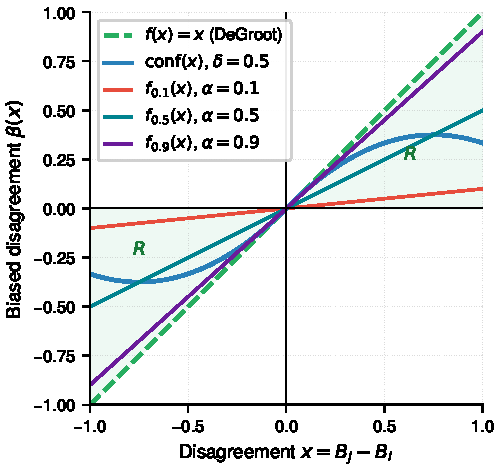
\includegraphics[width=0.54\textwidth]{bias_functions_scaled_family.pdf}
  \caption{Bias functions on $S=[-1,1]^2$.
    The identity $f(x)=x$ (DeGroot, green) marks the boundary between
    the Malleability region $M$ and the Receptive-Resistant region $R$.
    The confirmation bias $\mathrm{conf}(x)$ (blue,~\cite{Alvim2024})
    exhibits nonlinear resistance to distant opinions.
    Three members of $\mathcal{F}_\alpha$ are shown with
    $\alpha\in\{0.1,0.5,0.9\}$ (magenta, cyan, dark-red).
    In the first quadrant all scaled functions lie strictly below the
    identity, and in the third quadrant strictly above it, confirming
    membership in $R$}
  \label{fig:bias-functions-scaled-family}
\end{figure}

\begin{lemma}[Scaled linear biases lie in $R$]\label{lem:in-R}
  For every $\alpha\in(0,1)$, $f_\alpha\in R$.
\end{lemma}

\begin{proof}
  For $x>0$: $f_\alpha(x)=\alpha x\in(0,x)$, so $(x,f_\alpha(x))\in R$.
  For $x<0$: $f_\alpha(x)=\alpha x\in(x,0)$, so $(x,f_\alpha(x))\in R$.
  For $x=0$: $f_\alpha(0)=0$, so $(0,0)\in R$.
\end{proof}

By Lemma~\ref{lem:in-R}, all results of
Section~\ref{sec:analysis-structure} apply uniformly to
$\mathcal{F}_\alpha$.  Moreover, each $f_\alpha$ induces a
\emph{contraction} on the opinion spread
$R_t=\max(\mathbf{B}^t)-\min(\mathbf{B}^t)$.

\begin{restatable}[Geometric decay of opinion spread]{lemma}{geomDecay}
\label{lem:contraction}
  Let $(G,\mathbf{B}^0,\mathbf{S}^0,\mu_G)$ be a \CBSOMminus\ model
  on a clique with $n\ge 2$, with $\beta_{i,j}=f_{\alpha_{i,j}}$ for
  all edges. Let
  $\alpha_{\min}=\min_{(j,i)\in E}\alpha_{i,j}$ and
  $I_{\min}=\min_{(j,i)\in E}I_{ji}$.
  Then for every $\varepsilon>0$ there exists $t\in\mathbb{N}$ such
  that $R_t < \varepsilon$.
\end{restatable}

\begin{proof}[Proof sketch]
  Each round in which a vocal neighbor $j$ influences the max-agent $i$
  decreases the maximum by at least $I_{\min}\cdot\alpha_{\min}\cdot R_t$,
  since all terms in the update of the max-agent are non-positive.
  By Corollary~\ref{cor:no-perpetual-silence}, such events occur
  infinitely often.  The full proof (in Appendix~\ref{app:proofs})
  also handles the case where the min-agent is persistently silent,
  showing its opinion is pulled toward the maximum by vocal agents,
  again forcing $R_t\to 0$.
\end{proof}

% ===================================================================
\FloatBarrier
\subsection{Consensus in Clique Graphs}
\label{sec:consensus-cliques}

% -------------------------------------------------------------------
\subsubsection{Cliques with \texorpdfstring{$n\ge 3$}{n >= 3}}

\begin{restatable}[Consensus in \CBSOMminus\ cliques with $n\ge 3$]{theorem}{cbsomConsensus}
\label{thm:cbsom-consensus-n3}
  Let $(G,\mathbf{B}^0,\mathbf{S}^0,\mu_G)$ be a \CBSOMminus\ model
  on an $n$-agent clique with $n\ge 3$ and
  $\beta_{i,j}=f_{\alpha_{i,j}}\in\mathcal{F}_\alpha$ for all edges.
  Then all agents converge to consensus.
\end{restatable}

\begin{proof}[Proof sketch]
  By Theorem~\ref{thm:cbsom-limits}, limits $U$ and $L$ exist.
  Suppose $U-L>0$.  By Lemma~\ref{lem:contraction}, $R_t<U-L$ for
  some $t$; yet Corollary~\ref{cor:cbsom-mono} requires
  $R_t\ge U-L$ for all $t$: contradiction.  Hence $U=L$, and the
  Squeeze Theorem~\cite{Houshang2014} yields consensus.
  Full proof in Appendix~\ref{app:proofs}.
\end{proof}

\begin{remark}
  Theorem~\ref{thm:cbsom-consensus-n3} extends
  Aranda et al.'s consensus result for \SOMminus\
  cliques~\cite{aranda2024sound} (identity bias, $\alpha=1$) to the
  full scaled linear family $\mathcal{F}_\alpha$, and lifts
  Alvim et al.'s $R$-bias consensus
  result~\cite{Alvim2024} from the synchronous DeGroot setting to the
  Spiral-of-Silence setting.
\end{remark}

Figures~\ref{fig:clique3-conf} and~\ref{fig:clique3-scaled} illustrate
consensus convergence on a 3-agent clique under $\mathrm{conf}(x)$
and $f_\alpha$ biases, respectively.

\begin{figure}[!htbp]
  \centering
  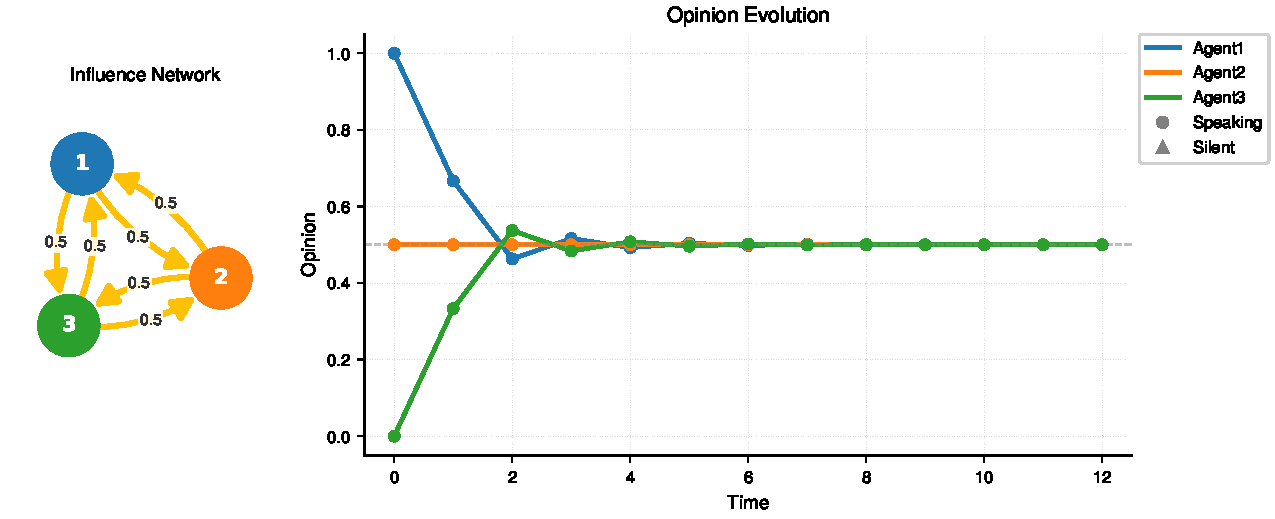
\includegraphics[width=0.95\textwidth]{FourthExperimentClique3Confirmation.pdf}
  \caption{Consensus on a 3-agent clique under \CBSOMminus\
    with $\mathrm{conf}(x)$ bias on all edges
    (Theorem~\ref{thm:cbsom-consensus-n3}).
    All directed edges carry influence weight $0.5$;
    initial beliefs are $\mathbf{B}^0=(1,0.5,0)$; $\tau_i=1$}
  \label{fig:clique3-conf}
\end{figure}

\begin{figure}[!htbp]
  \centering
  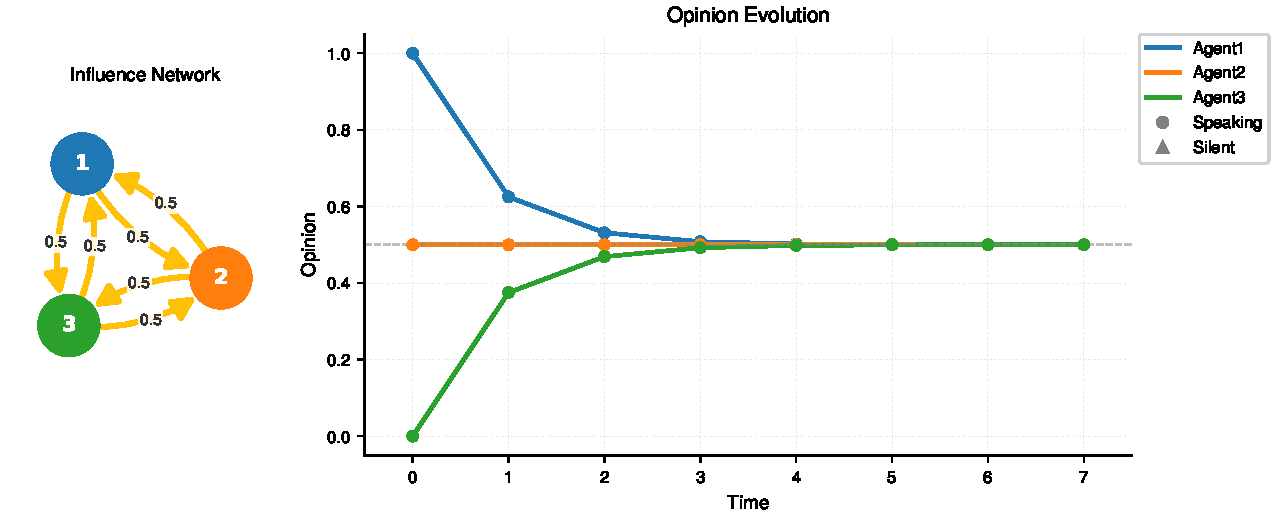
\includegraphics[width=0.95\textwidth]{FifthExperimentScaledConfirmationCliqueC.pdf}
  \caption{Consensus on a 3-agent clique under \CBSOMminus\
    with scaled linear bias $f_\alpha$, $\alpha=0.5$
    (Theorem~\ref{thm:cbsom-consensus-n3}).
    Same parameters as Figure~\ref{fig:clique3-conf}.
    $f_\alpha$ converges faster than $\mathrm{conf}(x)$ due to
    stronger linear attenuation of disagreement at all scales}
  \label{fig:clique3-scaled}
\end{figure}

% -------------------------------------------------------------------
\subsubsection{The Dyadic Case \texorpdfstring{$n=2$}{n = 2}}

The \SOMminus\ model fails to converge on two-agent cliques,
exhibiting period-2 oscillations~\cite{aranda2024sound}.
Figure~\ref{fig:som-n2-oscillation} illustrates this pathology:
with symmetric influence weights $I_{12}=I_{21}=1.0$ and
$\tau_i=1$, agents permanently alternate their beliefs between $0$
and $1$ without reaching any agreement.

\begin{figure}[!htbp]
  \centering%
  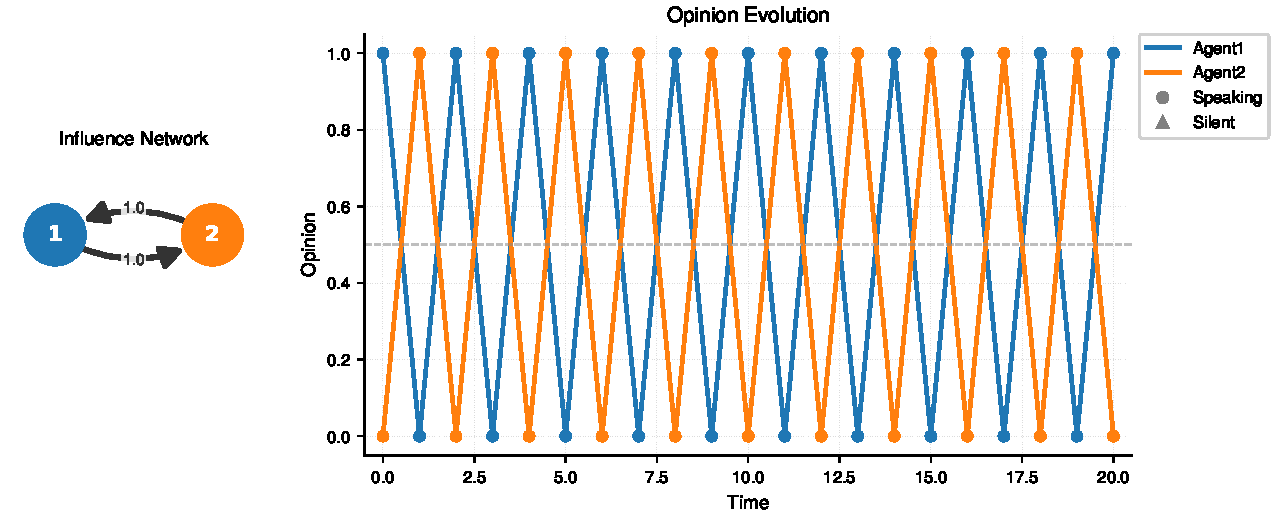
\includegraphics[width=0.95\textwidth]{FirstExperimentN2.pdf}
  \caption{Non-convergence counterexample for \SOMminus\ on a dyadic
    clique ($n=2$).
    Symmetric influence weights $I_{12}=I_{21}=1.0$,
    $\mathbf{B}^0=(1,0)$, $\tau_i=1$.
    Agents permanently oscillate between $0$ and $1$, alternating
    speaking and silent roles; consensus is never reached.
    This is the pathology that Theorem~\ref{thm:cbsom-consensus-n2}
    resolves by introducing $\mathcal{F}_\alpha$-biases}
  \label{fig:som-n2-oscillation}
\end{figure}

We now show that $\mathcal{F}_\alpha$-biases eliminate this pathology.

\begin{lemma}[Persistent vocality for $n=2$]\label{lem:vocal-n2}
  Consider \CBSOMminus\ on two agents $\{1,2\}$ with $\tau_1=\tau_2=1$.
  Then $S_1^t=S_2^t=1$ for all $t\in\mathbb{N}$.
\end{lemma}

\begin{proof}
  With $\tau_i=1$, the condition $|B_i^t-B_j^t|\le 1$ holds for all
  $t$ since opinions lie in $[0,1]$.  Hence every agent always satisfies
  the majority criterion and remains vocal.
\end{proof}

\begin{theorem}[Consensus under scaled linear biases for $n=2$]
\label{thm:cbsom-consensus-n2}
  Consider \CBSOMminus\ on a two-agent clique $\{1,2\}$ with
  $I_{21},I_{12}>0$, biases $\beta_{i,j}(x)=\alpha_{i,j}x$ with
  $\alpha_{i,j}\in(0,1)$, and $\tau_1=\tau_2=1$.
  Then both agents converge to consensus.
\end{theorem}

\begin{proof}
  By Lemma~\ref{lem:vocal-n2}, $S_j^t=1$ for all $t$.
  Let $\lambda_{12}=I_{21}\alpha_{1,2}$ and
  $\lambda_{21}=I_{12}\alpha_{2,1}$.
  Eq.~\eqref{eq:cbsom-minus-b} reduces to:
  \begin{align*}
    B_1^{t+1}&=(1-\lambda_{12})B_1^t+\lambda_{12}B_2^t,\\
    B_2^{t+1}&=\lambda_{21}B_1^t+(1-\lambda_{21})B_2^t.
  \end{align*}
  Let $D^t=B_1^t-B_2^t$.  Subtracting:
  $D^{t+1}=\gamma D^t$ where
  $\gamma=1-\lambda_{12}-\lambda_{21}$.
  Since $\alpha_{i,j}\in(0,1)$ and $I_{ji}>0$ for both edges,
  $\lambda_{12}=I_{21}\alpha_{1,2}\in(0,I_{21})$ and
  $\lambda_{21}=I_{12}\alpha_{2,1}\in(0,I_{12})$ are both strictly
  positive.  Hence $\lambda_{12}+\lambda_{21}\in(0,\,I_{21}+I_{12})$.
  Since $I_{12},I_{21}\le 1$ and $\alpha_{i,j}<1$,
  $\lambda_{12}+\lambda_{21}<2$; combined with strict positivity,
  $\gamma=1-\lambda_{12}-\lambda_{21}\in(-1,1)$, so $|\gamma|<1$.
  Therefore $D^t=\gamma^t D^0\to 0$, and both agents converge to
  the same limit $v\in[0,1]$.
\end{proof}

\begin{remark}[Asymmetric bias case]\label{rem:n2-asymmetric}
  Theorem~\ref{thm:cbsom-consensus-n2} requires $\alpha_{i,j}\in(0,1)$
  for \emph{both} directed edges.  The asymmetric case---one edge with
  $\alpha=1$ (identity, no bias) and one with $\alpha\in(0,1)$---falls
  outside the stated hypotheses but is conjectured to converge; we
  leave a formal treatment for future work.
\end{remark}

\begin{remark}[Recovery of the $n=2$ pathology]
\label{rem:n2-recovery}
  The period-2 oscillation of \SOMminus~\cite{aranda2024sound}
  corresponds to $\gamma=-1$, requiring
  $\lambda_{12}+\lambda_{21}=2$.
  With $\alpha_{i,j}\in(0,1)$, $\lambda_{ij}=I_{ji}\alpha_{i,j}<1$
  strictly, so $|\gamma|<1$ always.
  In the symmetric case ($I_{12}=I_{21}=I$,
  $\alpha_{1,2}=\alpha_{2,1}=\alpha$),
  the contraction rate is $\gamma=1-2\alpha I$:
  larger $\alpha$ produces oscillatory (but still convergent) dynamics,
  while smaller $\alpha$ yields monotone smooth convergence.
\end{remark}

Figures~\ref{fig:n2-alpha01} and~\ref{fig:n2-alpha09} illustrate how
$\alpha$ controls the qualitative character of convergence in
Case~2 of Theorem~\ref{thm:cbsom-consensus-n2}.

\begin{figure}[!htbp]
  \centering
  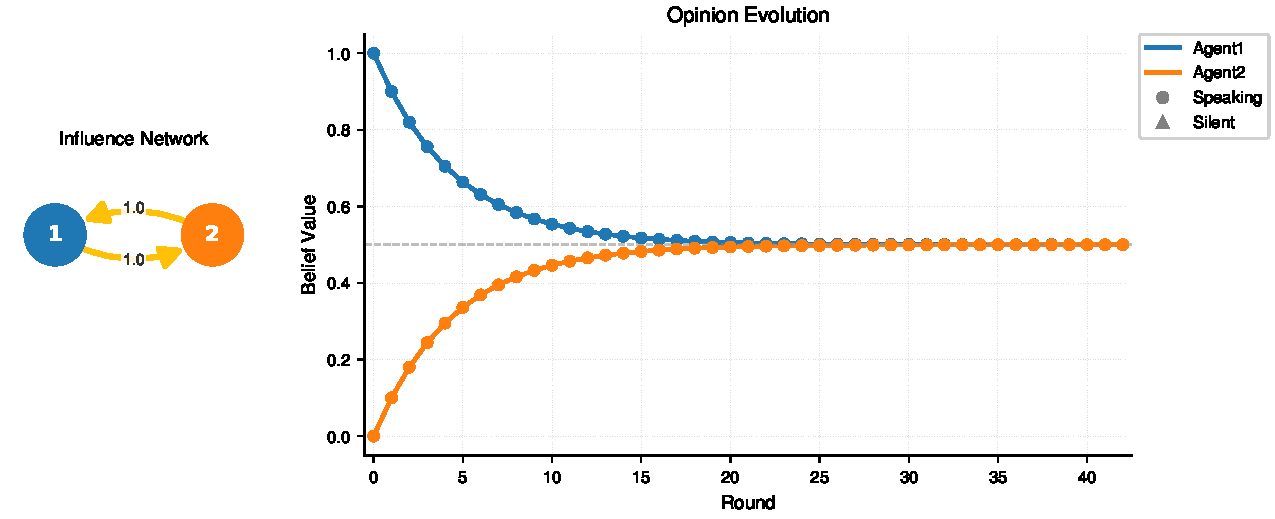
\includegraphics[width=0.95\textwidth]{2alpha01.pdf}
  \caption{Consensus on a two-agent clique under \CBSOMminus\ with
    scaled linear bias $f_\alpha$, $\alpha=0.1$
    (Case~2 of Theorem~\ref{thm:cbsom-consensus-n2}).
    Parameters: $I_{12}=I_{21}=1.0$, $\mathbf{B}^0=(1,0)$, $\tau_i=1$.
    With $\gamma=1-2\alpha I=0.8$ the opinion gap shrinks monotonically
    (``inverse trumpet'' profile)}
  \label{fig:n2-alpha01}
\end{figure}

\begin{figure}[!htbp]
  \centering
  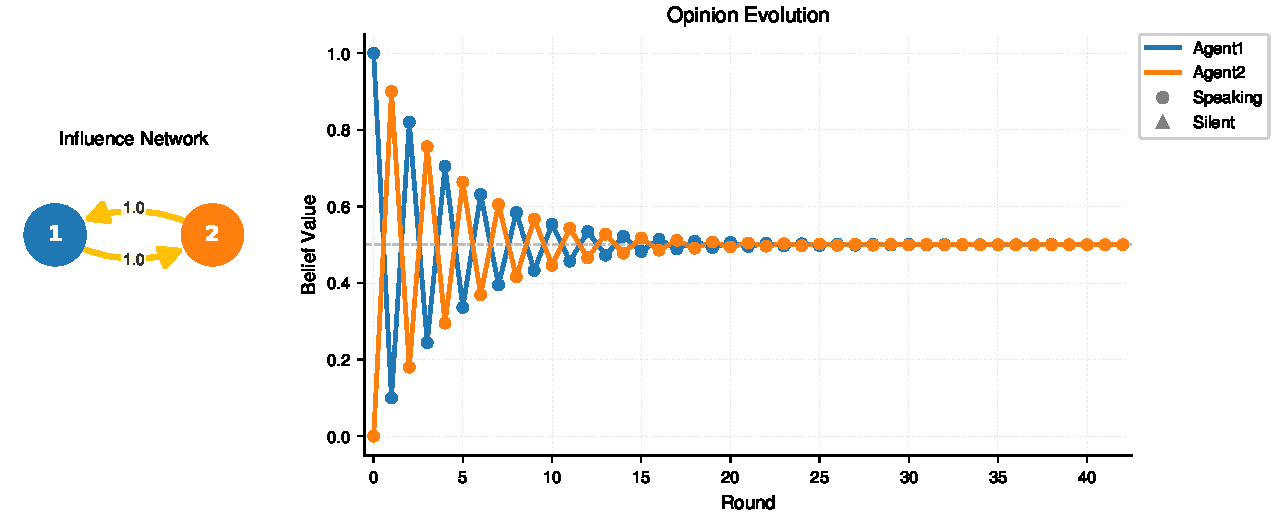
\includegraphics[width=0.95\textwidth]{2alpha09.pdf}
  \caption{Consensus on a two-agent clique under \CBSOMminus\ with
    scaled linear bias $f_\alpha$, $\alpha=0.9$.
    Same parameters as Figure~\ref{fig:n2-alpha01}.
    With $\gamma=-0.8$ the gap contracts oscillatorily but with
    strictly decreasing amplitude, reminiscent of the \SOMminus\
    pathology (Figure~\ref{fig:som-n2-oscillation}) but convergent.
    The special case $\alpha=0.5$ reaches consensus
    exactly at round~1: $B_1^1=B_2^1=0.5$}
  \label{fig:n2-alpha09}
\end{figure}

% ===================================================================
\FloatBarrier
\subsection{Summary}
\label{sec:analysis-summary}

Table~\ref{tab:consensus-summary} summarizes the consensus landscape
across models and clique sizes.

\begin{table}[ht]
\centering%
\caption{Consensus in clique graphs: \SOMminus\ vs.\ \CBSOMminus\
  with $\mathcal{F}_\alpha$-biases}
\label{tab:consensus-summary}
\begin{tabular}{lcc}
  \hline
  \textbf{Model} & \textbf{$n=2$} & \textbf{$n\ge 3$}\\
  \hline
  \SOMminus~\cite{aranda2024sound}
    & oscillates & converges\\
  \CBSOMminus\ $+$ $\mathcal{F}_\alpha$ \emph{(this work)}
    & converges & converges\\
  \hline
\end{tabular}
\end{table}

The decoupling between bias and silence---formalized in
Lemma~\ref{lem:no-perpetual-silence}---is the structural key: silence
determines \emph{who speaks} while bias determines \emph{how the
spoken opinion is absorbed}.  Consensus emerges from the joint action
of the contraction induced by $\mathcal{F}_\alpha$
(Lemma~\ref{lem:contraction}) and the impossibility of perpetual
silence (Corollary~\ref{cor:no-perpetual-silence}).

\section{Experimental Evaluation}
\label{sec:experiments}

The results of Section~\ref{sec:analysis} cover \CBSOMminus\ on cliques
with scaled linear biases. In this section, we study through simulation
the settings that those results do not cover: scale-free graphs,
biases outside the region $R$, mixtures of biases, and the memory-based
model \CBSOMplus. We run both models across eight network sizes and a
full range of connectivity levels. Our goals are threefold:
(i)~to test whether only $R$-region bias functions support consensus;
(ii)~to quantify the joint effect of network size and density on the
consensus threshold; and (iii)~to characterize how memory changes these
effects.

% -------------------------------------------------------------------
\subsection{Simulation Setup}
\label{sec:exp-setup}

The simulator generates scale-free graphs by preferential attachment
with degree-distribution exponent $\gamma=2.5$. This value lies in the
empirically documented range for scale-free social
networks~\cite{Barabasi1999,Newman2003,Clauset2009}.
The parameter grid is:
\begin{enumerate}
  \item \textbf{Network sizes:}
        $n \in \{10, 50, 100, 500, 10^3, 10^4, 10^5, 10^6\}$.
  \item \textbf{Density:} $1$--$9$ average neighbors per agent.
  \item \textbf{Bias types:} Unbiased ($\SOMminus$/$\SOMplus$),
        Confirmation, Backfire, and Authority
        (all under $\CBSOMminus$ or $\CBSOMplus$).
  \item \textbf{Runs per configuration:}
        $1{,}000$ ($n \le 10^3$); $500$ ($n=10^4$);
        $50$ ($n=10^5$); $10$ ($n=10^6$).
  \item \textbf{Convergence criterion:}
        opinion spread $\max_i B_i^t - \min_i B_i^t < 10^{-3}$;
        iteration cap $1{,}000$ rounds.
  \item \textbf{Initial opinions:} $B_i^0\sim\mathcal{U}[0,1]$.
\end{enumerate}

\paragraph{Metrics.}
The \emph{Consensus Rate} $\mathrm{CR}$
is the fraction of runs that converge. The
\emph{Mean Convergence Time} $\mathrm{MCT}$ is the average number of
rounds over converging runs. We report $\mathrm{CR}$ throughout.\footnote{All experiments were run on an Intel~i7-1255U machine with 32\,GB RAM and a 512\,GB NVMe SSD.}

% -------------------------------------------------------------------
\subsection{Uniform Networks}
\label{sec:exp-uniform}

A \emph{uniform} network assigns the same bias type to every edge and
the same silence model to every agent. This setting isolates the
contribution of each bias region before we consider mixtures.

\paragraph{Memoryless dynamics ($\CBSOMminus$).}
Figure~\ref{fig:heatmap-uniform} (top row) summarizes the full
$(n,\text{density})$ grid. Both $\SOMminus$ and $\CBSOMminus$
(Confirmation) move from near-zero to near-$100\%$ consensus as
density increases. The Confirmation panel is always at least as light
as the $\SOMminus$ panel: $R$-region biases act as
\emph{consensus accelerators}. The advantage is largest at the
transition. At $n=10^6$ and density~4, the consensus rate is $70\%$ for
$\CBSOMminus$ (Confirmation) and $10\%$ for $\SOMminus$
(Figure~\ref{fig:curves}).
The Backfire panel is uniformly black, i.e., there is no consensus at any
scale or density. Authority also yields zero consensus, except for
negligible events in a 10-agent network. This pattern is consistent with
Theorems~\ref{thm:cbsom-consensus-n3} and~\ref{thm:cbsom-consensus-n2},
which guarantee consensus only for $R$-region biases. However, at
$n=10^6$ the sample is too small (10 runs per configuration) to assert
an absolute dichotomy; these results should be taken as indicative.

The consensus threshold grows sub-linearly with $n$. Density~2 suffices
for $n \le 100$, density~3--4 for $n \in [10^3, 10^5]$, and density~4--5
for $n=10^6$. Figure~\ref{fig:curves} shows the corresponding rightward
shift of the S-curve: as $n$ increases, the transition from zero to full
consensus requires one or two additional neighbors per agent. Once the
threshold is crossed, the consensus rate approaches $100\%$. This holds
in all observed runs for $n \le 10^5$, where each configuration has at
least 50 runs.

\paragraph{Memory-based dynamics ($\CBSOMplus$).}
The bottom row of Figure~\ref{fig:heatmap-uniform} differs markedly
from the top row. For $n \le 100$, the Confirmation panel retains a faint
non-zero region at low densities (e.g., $19.9\%$ at $n=50$,
density~2), while $\SOMplus$ is already near zero.
For $n=500$, $\CBSOMplus$ (Confirmation) peaks at $4.9\%$; for
$n=1{,}000$, it falls to $3.8\%$ and is confined to densities $4$--$7$.
Beyond $n=10^4$, no memory-based configuration, including Confirmation,
reaches consensus in a single run at any density.
Figure~\ref{fig:memory-penalty} makes this collapse visible. The
Confirmation advantage that sustains high consensus in the left panel
($\CBSOMminus$) disappears in the right panel ($\CBSOMplus$)
as $n$ grows.

\begin{figure}[!htbp]
  \centering
  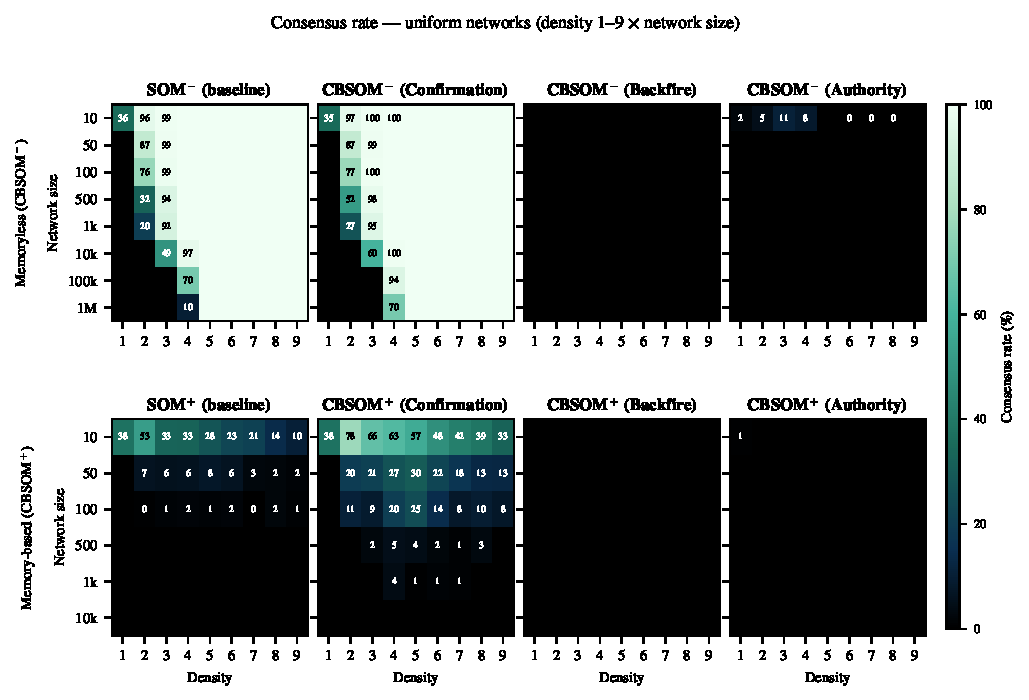
\includegraphics[width=0.85\columnwidth]{fig_heatmap_uniform.pdf}
  \caption{Consensus rate (color, black~$=0\%$, near-white~$=100\%$)
    for \emph{uniform} networks over the full $(n, \text{density})$ grid.
    \textbf{Top row} ($\CBSOMminus$, memoryless): $\SOMminus$ and
    Confirmation transition to near-white at moderate density across all
    eight scales; Backfire and Authority are uniformly black.
    \textbf{Bottom row} ($\CBSOMplus$, memory-based): only Confirmation
    retains a faint non-zero patch for $n \le 100$ and low density;
    all other configurations yield zero}
  \label{fig:heatmap-uniform}
\end{figure}

\begin{figure}[!htbp]
  \centering
  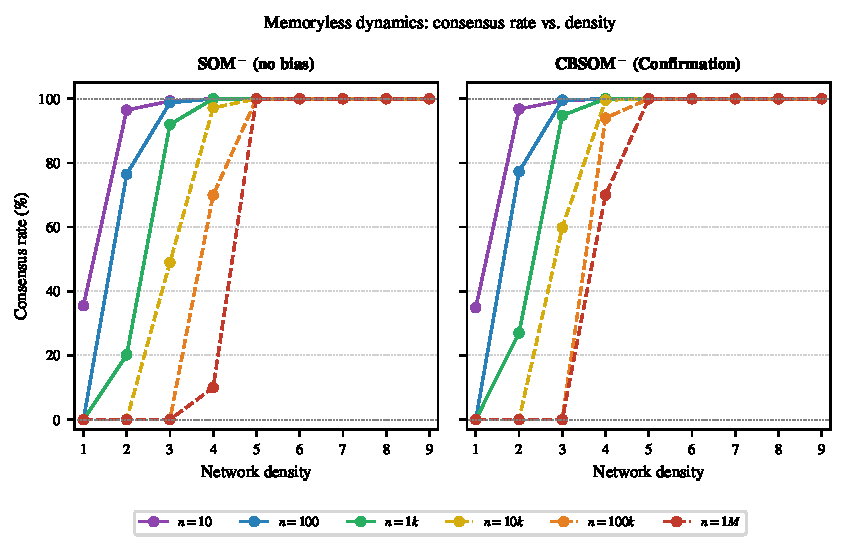
\includegraphics[width=0.85\columnwidth]{fig_consensus_curves.pdf}
  \caption{Consensus rate vs.\ density for $\SOMminus$ (left) and
    $\CBSOMminus$ (Confirmation, right) at six representative scales.
    Confirmation (right) saturates one density unit earlier than $\SOMminus$
    (left) for the same $n$, and the S-curve shifts rightward as
    $n$ grows, reflecting the sub-linear increase in the consensus
    threshold with network size}
  \label{fig:curves}
\end{figure}

\begin{figure}[!htbp]
  \centering
  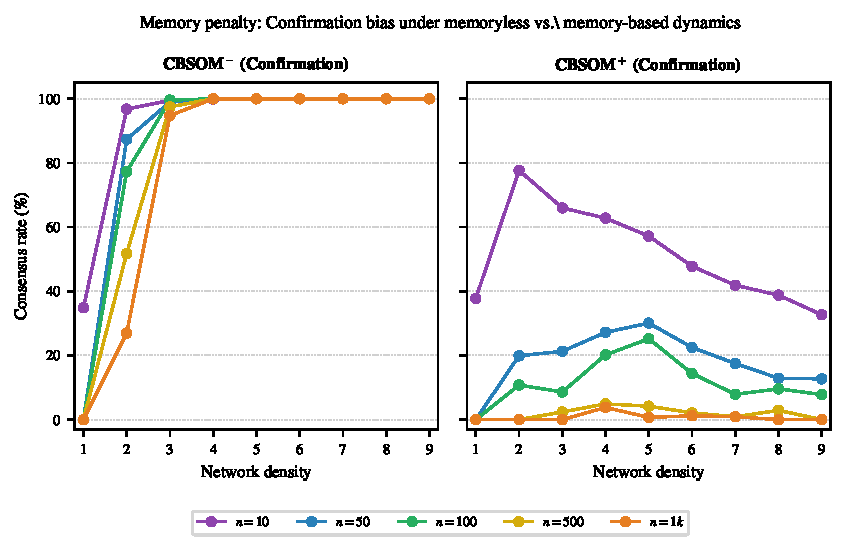
\includegraphics[width=0.85\columnwidth]{fig_memory_penalty.pdf}
  \caption{Memory penalty under Confirmation bias: $\CBSOMminus$ (left)
    versus $\CBSOMplus$ (right).  In the memoryless model consensus is
    robust across all $n \le 10^3$; in the memory-based model it
    collapses rapidly as $n$ grows, vanishing entirely for $n=1{,}000$
    at high densities}
  \label{fig:memory-penalty}
\end{figure}

% -------------------------------------------------------------------
\FloatBarrier
\subsection{Non-Uniform Networks}
\label{sec:exp-nonuniform}

\emph{Non-uniform} networks assign different bias types to different
edges. We consider four mixed configurations; the proportions refer to
fractions of edges:
\begin{enumerate}
  \item[(i)]  $\SOMminus+\CBSOMminus(\text{Conf.})$, $70\%/30\%$
  \item[(ii)] $\CBSOMminus(\text{Conf.})+\CBSOMminus(\text{Back.})$,
              $80\%/20\%$
  \item[(iii)]$\CBSOMminus(\text{Conf.})+\CBSOMminus(\text{Auth.})$,
              $60\%/40\%$
  \item[(iv)] $\SOMminus+\CBSOMminus(\text{Back.})$, $90\%/10\%$
\end{enumerate}

\paragraph{Rationale for the choice of proportions.}
We selected the four configurations heuristically. They are not
calibrated to measured distributions of cognitive biases in real social
networks; to our knowledge, no such data exist at the resolution
required to assign a bias type to each edge. Instead, the proportions
follow from the uniform-network results of Section~\ref{sec:exp-uniform}
and from an observation already present in the Spiral-of-Silence model
of Aranda et al.~\cite{aranda2024sound}: consensus is structurally
difficult to achieve even without cognitive biases.

Uniform Backfire and Authority configurations yield zero consensus at
every scale and density. Pure non-$R$ configurations therefore offer no
interesting boundary to explore. The relevant question is how small a
disruptive minority suffices to destroy consensus that would otherwise
form. Configuration~(iv) ($10\%$ Backfire) is a \emph{contamination}
scenario: it asks whether a marginal fraction of adversarial edges can
override an otherwise consensus-forming majority. Configuration~(ii)
($20\%$ Backfire) raises the disruptive load but keeps a
receptive-resistant supermajority. It probes the point at which updating
dominated by $\mathrm{conf}(x)$ can no longer absorb the opposing force.
Configuration~(iii) ($40\%$ Authority) places the two regimes in
near-balance. It tests whether substantial hierarchical influence is
compatible with global agreement. Finally, configuration~(i)
($30\%$ $\mathrm{conf}(x)$, $70\%$ unbiased) asks the complementary
question: can a receptive-resistant minority \emph{rescue} or amplify
consensus in an unbiased network that already struggles to converge at
large scales?

The proportions thus span a gradient from marginal perturbation to
near-parity. They cover regimes in which consensus is expected to be
fragile, recoverable, or structurally precluded. Bias distributions
that vary by agent role, community membership, or time may shift these
thresholds. We leave the calibration of proportions to empirical
social-network data for future work.

\paragraph{Memoryless dynamics.}
Figure~\ref{fig:heatmap-nonuniform} shows the results.
Configuration~(i) closely mirrors the uniform Confirmation baseline.
Consensus reaches $97\%$ by density~3 for $n=500$, and the transition
shifts rightward to density~5 only for $n=10^6$. Hence mixing
confirmation-biased and unbiased edges in a $30/70$ proportion
preserves the robustness of consensus.

Configurations (ii)--(iv) collapse to near-zero consensus at every
scale. At $n=100$, configurations (ii) and (iv) produce at most
$2\%$--$3\%$ consensus across all densities; for $n \ge 500$, consensus
is identically zero. A $10\%$ share of Backfire edges
(configuration~iv) suffices to eliminate consensus that would otherwise
occur in almost every run. This \emph{robustness asymmetry} has a clear
direction. Edges in $R$ act as consensus catalysts, whereas edges
outside $R$ prevent consensus, and a surrounding majority of $R$-region
edges cannot neutralize them.

\paragraph{Memory-based dynamics.}
In non-uniform memory-based networks, consensus is essentially absent.
The $\SOMplus+\CBSOMplus(\text{Conf.})$ $70/30$ mixture produces
sporadic consensus only for $n \le 100$ (at most $30\%$, density~4).
For $n \ge 500$, no run converges under any mixed memory-based
configuration. Memory thus amplifies the disruptive effect of non-$R$
edges: at scale, we observed no consensus at all.

\begin{figure}[!htbp]
  \centering
  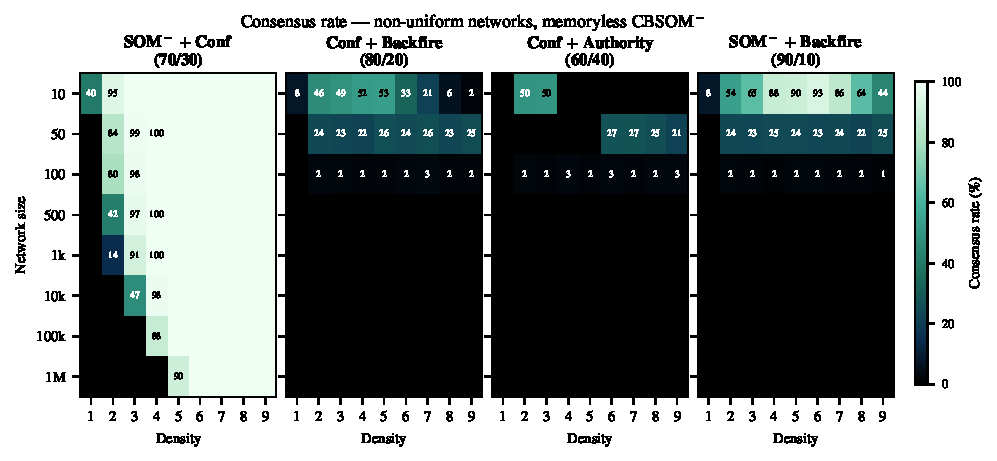
\includegraphics[width=\columnwidth]{fig_heatmap_nonuniform.pdf}
  \caption{Consensus rate for \emph{non-uniform} memoryless networks
    ($\CBSOMminus$) over the full $(n, \text{density})$ grid.  Only the
    $\SOMminus+\CBSOMminus(\text{Conf.})$ $70/30$ mixture (leftmost panel)
    achieves near-$100\%$ consensus at moderate density. Every
    configuration that contains Backfire or Authority edges collapses to
    near-zero consensus at every scale. This illustrates the robustness
    asymmetry between influence inside and outside the region $R$}
  \label{fig:heatmap-nonuniform}
\end{figure}

% -------------------------------------------------------------------
\FloatBarrier
\subsection{Relative Density}
\label{sec:exp-relative}

The experiments in Sections~\ref{sec:exp-uniform}
and~\ref{sec:exp-nonuniform} measure connectivity by an absolute
neighbor count $k\in\{1,\dots,9\}$. The same count represents very
different levels of social exposure as the network grows.
To assess whether the observed effects depend on this choice, we add a
\emph{relative-density} analysis. In it, the neighborhood of each agent
is a fixed fraction
$\rho\in\{10\%,\,25\%,\,50\%,\,75\%,\,100\%\}$ of the maximum
feasible degree $n-1$.
The $100\%$ condition is the complete-graph limit: every agent
interacts with every other.
Experiments cover $n\in\{100,\,1{,}000,\,10{,}000\}$ with the same
run counts and convergence criterion as Section~\ref{sec:exp-setup}.

Figures~\ref{fig:heatmap-rel-uniform} and~\ref{fig:heatmap-rel-nonuniform}
summarize the four scenarios, one per figure row.

\paragraph{Uniform memoryless (Figure~\ref{fig:heatmap-rel-uniform}, top row).}
$\SOMminus$ and $\CBSOMminus$ (Confirmation) achieve $100\%$ consensus
at every relative density and every tested scale, including the
sparsest configuration ($\rho=10\%$, $n=10{,}000$,
i.e.\ $\approx\!1{,}000$ neighbors per agent).
Backfire and Authority yield $0\%$ everywhere.
The all-white and all-black panels indicate that, in this range, the
bias-region dichotomy depends on the bias type alone and not on the
connectivity level.

\paragraph{Uniform memory-based (Figure~\ref{fig:heatmap-rel-uniform}, bottom row).}
All cells are black for $n\ge 1{,}000$ across all configurations and
all relative densities, including the complete-graph limit
($\rho=100\%$).
The only non-zero values appear at $n=100$: $11.1\%$ and $0.9\%$
for Conf\,+\,Backfire (80/20) at $\rho=10\%$ and $25\%$
respectively, and $0.1\%$ for SOM$^+$\,+\,Confirmation (70/30) at
$\rho=10\%$; all vanish at $\rho\ge 50\%$.

\paragraph{Non-uniform memoryless (Figure~\ref{fig:heatmap-rel-nonuniform}, top row).}
The SOM$^-$\,+\,Conf (70/30) column is entirely white: mixing a $30\%$
confirmation minority with an unbiased majority preserves $100\%$
consensus at every scale and every relative density.
The three disruptive mixtures annotate small non-zero values
($1.4$--$3.0\%$) only at $n=100$; for $n\ge 1{,}000$ they are
identically zero regardless of $\rho$.

\paragraph{Non-uniform memory-based (Figure~\ref{fig:heatmap-rel-nonuniform}, bottom row).}
The entire row is black: zero consensus for all configurations,
all three scales, and all relative densities up to the complete graph.

Together, the two memory-based scenarios sharpen the memory-barrier
conclusion of Section~\ref{sec:exp-discussion}. Increasing connectivity,
up to and including the complete graph, does not overcome the
suppression of consensus under $\CBSOMplus$. The barrier is therefore
structural rather than a threshold effect.

\begin{figure}[!htbp]
  \centering
  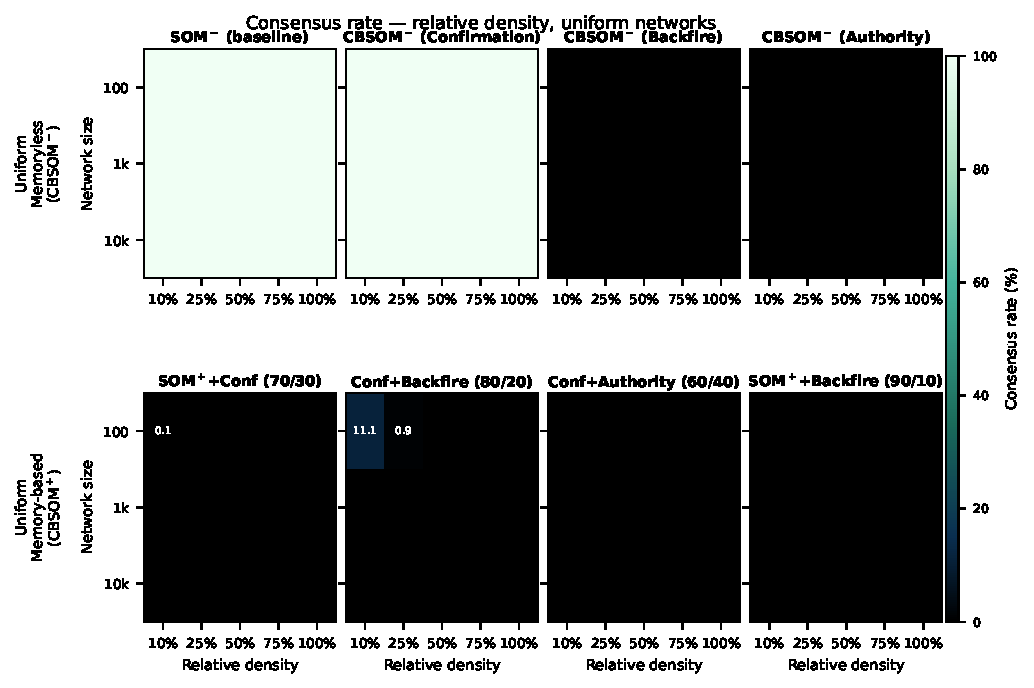
\includegraphics[width=0.85\columnwidth]{fig_heatmap_relative_density_uniform.pdf}
  \caption{Consensus rate (color scale as in
    Figures~\ref{fig:heatmap-uniform}--\ref{fig:heatmap-nonuniform})
    for relative-density experiments on \emph{uniform} networks
    ($\rho\in\{10\%,25\%,50\%,75\%,100\%\}$,
    $n\in\{100,\,1\mathrm{k},\,10\mathrm{k}\}$).
    \textbf{Top row} (memoryless): SOM$^-$ and Confirmation are
    near-white at every cell; Backfire and Authority are uniformly
    black; the bias dichotomy does not depend on density.
    \textbf{Bottom row} (memory-based): all black for $n\ge 1{,}000$
    at every $\rho$, including the complete graph ($\rho=100\%$);
    non-zero values appear only at $n=100$, $\rho\le 25\%$
    (11.1\% and 0.9\% for Conf+Backfire; 0.1\% for SOM$^+$+Conf)}
  \label{fig:heatmap-rel-uniform}
\end{figure}

\begin{figure}[!htbp]
  \centering
  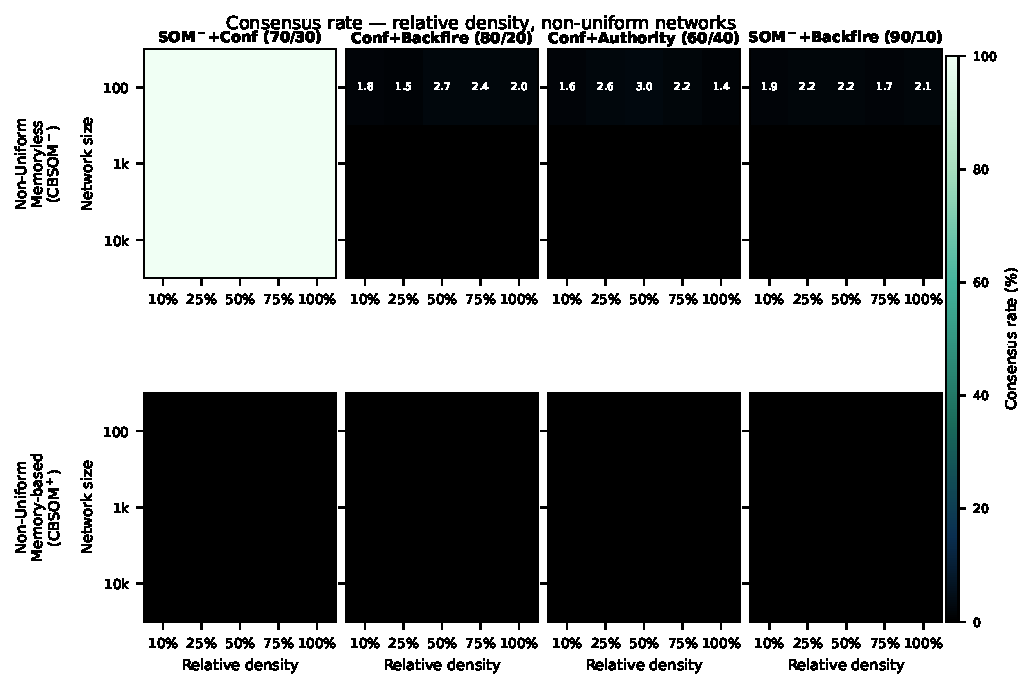
\includegraphics[width=0.85\columnwidth]{fig_heatmap_relative_density_nonuniform.pdf}
  \caption{Consensus rate for relative-density experiments on
    \emph{non-uniform} networks (same color scale and parameter
    grid as Figure~\ref{fig:heatmap-rel-uniform}).
    \textbf{Top row} (memoryless): the SOM$^-$+Conf (70/30) column
    is uniformly near-white at all scales and relative densities;
    disruptive mixtures annotate marginal values ($\le 3\%$) only
    at $n=100$, vanishing for $n\ge 1{,}000$.
    \textbf{Bottom row} (memory-based): uniformly black across all
    configurations, scales, and relative densities, including the
    complete-graph limit ($\rho=100\%$)}
  \label{fig:heatmap-rel-nonuniform}
\end{figure}

% -------------------------------------------------------------------
\FloatBarrier
\subsection{Discussion}
\label{sec:exp-discussion}

Three empirical findings summarize the experimental evidence:

\begin{enumerate}
  \item \textbf{Bias-region dichotomy.}
    $R$-region biases (Confirmation) yield $\mathrm{CR}$ approaching
    $100\%$ at sufficient density for $n\le 10^5$ (at least 50 runs per
    configuration). At $n=10^6$ (10~runs), all Confirmation runs converge
    at density~$\ge 5$, but the sample is too small to assert
    $\mathrm{CR}=100\%$ unconditionally.
    Non-$R$ biases (Backfire, Authority) yield $\mathrm{CR}=0\%$
    in all observed runs at every scale and density tested.

  \item \textbf{Sub-linear consensus threshold.}
    The critical density grows from $2$ (small networks) to $4$--$5$
    ($n=10^6$), spanning only $3$ units across eight orders of
    magnitude of network size. The threshold under Confirmation is
    consistently one unit lower than under the unbiased $\SOMminus$
    baseline.

  \item \textbf{Memory as a structural barrier.}
    Memory-based dynamics ($\SOMplus$, $\CBSOMplus$) almost entirely
    suppress consensus. Even Confirmation retains non-zero
    $\mathrm{CR}$ only at $n \le 1{,}000$. In non-uniform
    settings, an $R$-region majority cannot compensate for the path
    dependence induced by memory beyond $n=100$.
\end{enumerate}

\paragraph{Data and code availability.}
The Scala/Akka simulator used to produce the results reported in this
section is publicly available at
\url{https://github.com/juanmarcosdev/belief_evolution_simulator}.

\section{Conclusions and Related Work}
\label{sec:conclusions}

\subsection{Conclusions}

We introduced \CBSOMminus\ and \CBSOMplus, two extensions of the
Spiral-of-Silence opinion models of~\cite{aranda2024sound}
that incorporate cognitive bias functions into the belief-update rule.
We identified the Receptive-Resistant region~$R$ as the structural
condition under which bias-augmented dynamics preserve the key structural
properties of the base model: scaled linear $R$-biases guarantee consensus
on cliques for all $n \geq 2$, while backfire and authority biases
consistently prevent it in all simulated scenarios.
To our knowledge, this is the first work to embed cognitive bias functions
into a Spiral-of-Silence framework and to provide formal consensus
guarantees for the resulting models.
The theoretical results are corroborated by large-scale simulations over
networks ranging from $10$ to $10^6$ agents, confirming the bias-region
dichotomy observed empirically, a sub-linear growth of the critical density
threshold with network size, and the structural consensus barrier
introduced by memory-based dynamics.

In future work, we plan to extend the consensus analysis beyond cliques to
arbitrary strongly-connected graphs.
We also plan to extend the framework to dynamic network topologies, where
the influence graph evolves over time, and to confidence-based silence
formulations, not yet studied under cognitive bias.
Finally, coupling the simulation framework with empirical social network
data would allow partial model validation and the tuning of bias parameters
to improve the predictive power of the models for real-world opinion
polarization phenomena.

\subsection{Related Work}

Alvim et al.~\cite{Alvim2024} introduce the bias region taxonomy---receptive-resistant,
malleable, backfire, and insular---used throughout this paper, and prove
that continuous $R$-region bias functions guarantee consensus in synchronous
DeGroot dynamics on strongly connected graphs.
Our work builds directly on this framework: Theorem~\ref{thm:cbsom-consensus-n3}
lifts the $R$-bias consensus guarantee from the synchronous DeGroot setting to the
Spiral-of-Silence setting, where the silence mechanism introduces a
structural decoupling between bias and silence decisions.
A key difference is that our consensus result is restricted to cliques under
the scaled linear subfamily $\mathcal{F}_\alpha$, whereas
Alvim et al.'s result holds for all continuous $R$-biases on
arbitrary strongly connected graphs; extending our result to that full
generality is an open problem.
Psychological foundations for the bias functions considered
here---confirmation, backfire, and authority---are discussed
in~\cite{Aronson2010}.

The Spiral-of-Silence models \SOMminus\ and \SOMplus\ were introduced
in~\cite{aranda2024sound}, which also studies their formal convergence
properties, establishing consensus in $n$-agent cliques for $n\ge 3$ and
the period-2 oscillation pathology on two-agent cliques.
Our Theorem~\ref{thm:cbsom-consensus-n2} resolves this pathology: any
scaled-linear bias $f_\alpha$ with $\alpha\in(0,1)$ breaks the oscillation
and restores consensus.
The memory-based model \CBSOMplus\ exhibits substantially lower consensus
rates than \CBSOMminus\ across all scales; this mirrors the behavior already
observed for \SOMplus\ in~\cite{aranda2024sound} and confirms that memory
acts as a structural barrier independent of the bias layer.

The structural decoupling identified in
Section~\ref{sec:analysis-structure}---the silence criterion of \CBSOMminus\
depends only on raw opinion proximity and not on bias-filtered values---means
that the consensus guarantees of~\cite{aranda2024sound} for \SOMminus\
extend naturally to \CBSOMminus\ with $R$-region biases: wherever the
silence dynamics create conditions for consensus in the base model, the bias
layer does not interfere with those conditions.
A comparable argument for \CBSOMplus\ remains open, as the memory layer
couples historical opinion values with the current silence decision in a
non-trivial way.


%% ================================================================
%% BACK MATTER (order as in the CLEIej template:
%% Acknowledgment -> References -> Appendix)
%% ================================================================
\FloatBarrier
\section*{Acknowledgment}
This work has been partially supported by the SGR project PROMUEVA
(BPIN 2021000100160) under the supervision of Minciencias (Ministerio de
Ciencia, Tecnolog\'{i}a e Innovaci\'{o}n, Colombia).

\bibliography{references}

\appendix
\section{Proofs}
\label{app:proofs}

This appendix contains the complete proofs of the
following results:

\begin{itemize}

  \item \hyperref[proof:cbsom-bounds]{%
    \textbf{Lemma~\ref{lem:cbsom-bounds}.}
    (Bounded opinions under \CBSOMminus)}

  \item \hyperref[proof:geom-decay]{%
    \textbf{Lemma~\ref{lem:contraction}.}
    (Geometric decay of opinion spread)}

  \item \hyperref[proof:consensus-n3]{%
    \textbf{Theorem~\ref{thm:cbsom-consensus-n3}.}
    (Consensus in \CBSOMminus\ cliques with $n\ge 3$)}

\end{itemize}



\cbsomBounds*

\begin{proof}\label{proof:cbsom-bounds}
  Let $M=\max(\mathbf{B}^t)$ and $m=\min(\mathbf{B}^t)$.
  Fix any agent $i\in A$.
  By Eq.~\eqref{eq:cbsom-minus-b}:
  \begin{equation}\label{eq:app-bounds-expand}
    B_i^{t+1}
    = B_i^t
      + \underbrace{\sum_{j\in N^t(i)}
          I_{ji}\cdot\beta_{i,j}(B_j^t - B_i^t)}_{=:\,\Sigma_i^t},
  \end{equation}
  where $N^t(i)=\{j\in N(i):S_j^t=1\}$.
  We partition $N^t(i)$ into three disjoint sets:
  \begin{align*}
    P^+_i &= \{j\in N^t(i): B_j^t > B_i^t\},\\
    P^-_i &= \{j\in N^t(i): B_j^t < B_i^t\},\\
    P^0_i &= \{j\in N^t(i): B_j^t = B_i^t\}.
  \end{align*}
  For every $j\in P^0_i$ the term is zero since $\beta_{i,j}(0)=0$
  (as $(0,0)\in R$).
  We analyse the non-zero contributions.

  \begin{pclaim}[Sign and magnitude of $\beta_{i,j}$ in $R$]
    \label{claim:R-properties}
    For $\beta_{i,j}\in R$ and $x\ne 0$:
    (a)~$\operatorname{sign}(\beta_{i,j}(x))=\operatorname{sign}(x)$;
    (b)~$|\beta_{i,j}(x)|\le|x|$.
  \end{pclaim}

  \noindent\emph{Proof of Claim.}
  Property~(a) follows from the definition of $R$
  (the graph of $\beta_{i,j}$ lies in the first and third quadrants
  of $S=[-1,1]^2$~\cite{Alvim2024}).
  Property~(b) follows from $|\beta_{i,j}(x)|\le|x|$ for all $(x,y)\in R$
  with $y=\beta_{i,j}(x)$~\cite{Alvim2024}. \hfill$\square$

  \medskip\noindent\textbf{Upper bound: $B_i^{t+1}\le M$.}

  By Claim~\ref{claim:R-properties}(a):
  each term with $j\in P^-_i$ satisfies
  $I_{ji}\cdot\beta_{i,j}(B_j^t-B_i^t)\le 0$.
  Dropping these non-positive contributions:
  \begin{align}
    \Sigma_i^t
    &\le \sum_{j\in P^+_i} I_{ji}\cdot\beta_{i,j}(B_j^t-B_i^t).
    \label{eq:app-sigma-upper}
  \end{align}
  By Claim~\ref{claim:R-properties}(b), for $j\in P^+_i$:
  $\beta_{i,j}(B_j^t-B_i^t)\le B_j^t-B_i^t$.
  Hence:
  \begin{align}
    B_i^{t+1}
    &\le B_i^t
      + \sum_{j\in P^+_i} I_{ji}(B_j^t-B_i^t)\notag\\
    &= B_i^t\!\Bigl(1-\!\sum_{j\in P^+_i}\!I_{ji}\Bigr)
      + \sum_{j\in P^+_i}\!I_{ji}\,B_j^t.
    \label{eq:app-upper-convex}
  \end{align}
  By row-stochasticity (Eq.~\eqref{eq:row-stochastic}),
  $\sum_{j\in P^+_i}I_{ji}\le
   \sum_{j\in N(i)\cup\{i\}}I_{ji}=1$,
  so the coefficient of $B_i^t$ is non-negative.
  Expression~\eqref{eq:app-upper-convex} is therefore a convex
  combination of $B_i^t$ and $\{B_j^t\}_{j\in P^+_i}$,
  all of which lie in $(-\infty,M]$.
  Therefore $B_i^{t+1}\le M$.

  \medskip\noindent\textbf{Lower bound: $B_i^{t+1}\ge m$.}

  By Claim~\ref{claim:R-properties}(a):
  each term with $j\in P^+_i$ satisfies
  $I_{ji}\cdot\beta_{i,j}(B_j^t-B_i^t)\ge 0$.
  Dropping these non-negative contributions:
  \begin{align}
    \Sigma_i^t
    &\ge \sum_{j\in P^-_i} I_{ji}\cdot\beta_{i,j}(B_j^t-B_i^t).
    \label{eq:app-sigma-lower}
  \end{align}
  By Claim~\ref{claim:R-properties}(b), for $j\in P^-_i$
  (where $B_j^t-B_i^t<0$): $\beta_{i,j}(B_j^t-B_i^t)\ge B_j^t-B_i^t$.
  Hence:
  \begin{align}
    B_i^{t+1}
    &\ge B_i^t
      + \sum_{j\in P^-_i} I_{ji}(B_j^t-B_i^t)\notag\\
    &= B_i^t\!\Bigl(1-\!\sum_{j\in P^-_i}\!I_{ji}\Bigr)
      + \sum_{j\in P^-_i}\!I_{ji}\,B_j^t.
    \label{eq:app-lower-convex}
  \end{align}
  By the same row-stochasticity argument,
  \eqref{eq:app-lower-convex} is a convex combination of $B_i^t$
  and $\{B_j^t\}_{j\in P^-_i}$, all of which lie in $[m,+\infty)$.
  Therefore $B_i^{t+1}\ge m$.

  \medskip\noindent Combining both bounds:
  $\min(\mathbf{B}^t)\le B_i^{t+1}\le\max(\mathbf{B}^t)$
  for all $i\in A$.
\end{proof}


\geomDecay*

This lemma states that, on a clique with scaled linear biases, the gap
between the highest and the lowest opinion becomes arbitrarily small. The
proof shows that steps in which the gap shrinks by a fixed fraction occur
infinitely often, even when some agents remain silent.

\begin{proof}\label{proof:geom-decay}
  Let $c=I_{\min}\cdot\alpha_{\min}\in(0,1)$,
  where $I_{\min}=\min_{(j,i)\in E}I_{ji}$ and
  $\alpha_{\min}=\min_{(j,i)\in E}\alpha_{i,j}$.
  Both are strictly positive by assumption.
  Let $\Delta_t=\max(\mathbf{B}^t)-\min(\mathbf{B}^t)$.
  By Corollary~\ref{cor:cbsom-mono}, $\{\Delta_t\}$ is non-increasing.

  We identify two disjoint types of steps and show that the second
  type occurs infinitely often, each time contracting $\Delta_t$ by a
  factor of at least $(1-c)$.

  \medskip
  \begin{pclaim}[Max-agent update on a clique with $\mathcal{F}_\alpha$-bias]
  \label{claim:max-drop}
    Let $G$ be a clique, $\beta_{i,j}=f_{\alpha_{i,j}}$, and
    $\Delta_t>0$.  If agent $i$ achieves $\max(\mathbf{B}^t)$ and
    there exists a vocal neighbor $j\in N^t(i)$ with
    $B_j^t < B_i^t$, then:
    \begin{equation}\label{eq:app-max-drop}
      \max(\mathbf{B}^{t+1})
      \;\le\;
      \max(\mathbf{B}^t) - c\cdot \Delta_t.
    \end{equation}
  \end{pclaim}

  \noindent\emph{Proof of Claim~\ref{claim:max-drop}.}
  Since $B_i^t=\max(\mathbf{B}^t)$, every vocal neighbor $k$ satisfies
  $B_k^t\le B_i^t$, so $B_k^t-B_i^t\le 0$ for all $k\in N^t(i)$.
  With $f_{\alpha_{i,k}}\in\mathcal{F}_\alpha\subset R$:
  $f_{\alpha_{i,k}}(B_k^t-B_i^t)=\alpha_{i,k}(B_k^t-B_i^t)\le 0$.
  Hence all terms in \eqref{eq:cbsom-minus-b} are non-positive, giving
  $B_i^{t+1}\le B_i^t$.  More precisely, isolating the $j$-term:
  \begin{align*}
    B_i^{t+1}
    &= B_i^t
      + \underbrace{I_{ji}\cdot\alpha_{i,j}\cdot(B_j^t-B_i^t)}_{<\;0}
      + \underbrace{\sum_{k\in N^t(i)\setminus\{j\}}
          I_{ki}\cdot\alpha_{i,k}\cdot(B_k^t-B_i^t)}_{\le\;0}\\
    &\le B_i^t - I_{ji}\cdot\alpha_{i,j}\cdot(B_i^t-B_j^t)\\
    &\le B_i^t - I_{\min}\cdot\alpha_{\min}\cdot(B_i^t-B_j^t).
  \end{align*}
  Since $j$ can be taken as the min-agent and
  $B_i^t-B_j^t\ge \Delta_t$:
  $B_i^{t+1}\le \max(\mathbf{B}^t)-c\cdot \Delta_t$.
  Together with $\max(\mathbf{B}^{t+1})\le B_i^{t+1}$
  (from Lemma~\ref{lem:cbsom-bounds}), Eq.~\eqref{eq:app-max-drop}
  follows. \hfill$\square$

  \medskip\noindent\textbf{Infinitely many contraction steps.}

  We call step $t$ \emph{productive} if $\Delta_t>0$ and there exists a
  vocal neighbor of the max-agent with strictly lower opinion.
  We show productive steps occur infinitely often.

  Suppose for contradiction that after some time $T$, no step is
  productive.  Then for all $t\ge T$ with $\Delta_t>0$, every vocal
  agent at time $t$ holds opinion $\max(\mathbf{B}^t)$.
  In this situation the min-agent $j$ (with $B_j^t<\max(\mathbf{B}^t)$)
  is silent at every $t\ge T$.
  Since $j$ is silent, $S_j^t=0$; but $j$ still updates its belief:
  \begin{equation}\label{eq:app-min-increase}
    B_j^{t+1}
    = B_j^t + \sum_{k\in N^t(j)}
        I_{kj}\cdot\alpha_{j,k}\cdot(B_k^t-B_j^t).
  \end{equation}
  Every vocal agent $k$ at time $t$ satisfies $B_k^t=\max(\mathbf{B}^t)\ge B_j^t$,
  so every term in \eqref{eq:app-min-increase} is non-negative.
  Hence $\{B_j^t\}_{t\ge T}$ is non-decreasing and bounded above by
  $\max(\mathbf{B}^T)$.  Let $v=\lim_{t\to\infty}B_j^t\ge B_j^T$.

  By Corollary~\ref{cor:no-perpetual-silence}, $N^t(j)\ne\emptyset$
  for infinitely many $t$.  Whenever $N^t(j)\ne\emptyset$ and
  $B_j^t<\max(\mathbf{B}^t)$, each vocal $k$ contributes a strictly
  positive term $I_{kj}\alpha_{j,k}(\max(\mathbf{B}^t)-B_j^t)>0$.
  By Lemma~\ref{lem:cbsom-bounds} and monotonicity
  (Corollary~\ref{cor:cbsom-mono}),
  $\max(\mathbf{B}^t)\ge U>L=\lim\min(\mathbf{B}^t)\ge B_j^t$
  (where we use Theorem~\ref{thm:cbsom-limits}).
  Hence the increment in \eqref{eq:app-min-increase} is bounded
  below by $I_{\min}\alpha_{\min}(U-B_j^t)>0$ at each such step,
  forcing $v\ge U$, i.e., $B_j^t\to U$.
  But $B_j^t$ is a (non-decreasing) sequence bounded above by $1$,
  and $B_j^t\to U$ means $\min(\mathbf{B}^t)\to U=\max(\mathbf{B}^t)$:
  $\Delta_t\to 0$, contradicting $\Delta_t>0$ for all $t\ge T$.

  Therefore productive steps occur infinitely often.

  \medskip\noindent\textbf{Geometric bound.}

  Let $\{t_k\}_{k\ge 0}$ be the (infinite) subsequence of productive
  steps.  By Claim~\ref{claim:max-drop} and
  Corollary~\ref{cor:cbsom-mono} (monotonicity of min):
  \[\Delta_{t_k+1}\le \Delta_{t_k}-c\cdot \Delta_{t_k}=(1-c)\,\Delta_{t_k}.\]
  Since $\Delta_t$ is non-increasing between productive steps:
  \[\Delta_{t_{k+1}}\le \Delta_{t_k+1}\le(1-c)\,\Delta_{t_k}.\]
  By induction:
  \[\Delta_{t_k}\le(1-c)^k\,\Delta_0.\]
  For every $\varepsilon>0$, choose $k$ large enough so that
  $(1-c)^k \Delta_0<\varepsilon$.
  Then $\Delta_{t_k}<\varepsilon$.
\end{proof}


\cbsomConsensus*

This theorem states that silence and scaled linear biases cannot prevent
agreement on cliques with at least three agents. The proof combines the
limits of the extreme opinions (Theorem~\ref{thm:cbsom-limits}) with the
contraction of the gap between them (Lemma~\ref{lem:contraction}).

\begin{proof}\label{proof:consensus-n3}
  By Theorem~\ref{thm:cbsom-limits}, the limits
  $U=\lim_{t\to\infty}\max(\mathbf{B}^t)$ and
  $L=\lim_{t\to\infty}\min(\mathbf{B}^t)$ exist in $[0,1]$ with $L\le U$.
  We show $U=L$ by contradiction.

  \medskip\noindent\textbf{Suppose $U-L=:\delta>0$.}

  Since $\max(\mathbf{B}^t)\to U$ and $\min(\mathbf{B}^t)\to L$,
  there exists $T_0\in\mathbb{N}$ such that for all $t\ge T_0$:
  \begin{equation}\label{eq:app-consensus-sandwich}
    \max(\mathbf{B}^t) \;\ge\; U-\tfrac{\delta}{4}
    \qquad\text{and}\qquad
    \min(\mathbf{B}^t) \;\le\; L+\tfrac{\delta}{4}.
  \end{equation}
  In particular, for all $t\ge T_0$:
  \begin{equation}\label{eq:app-Rt-lower}
    \Delta_t = \max(\mathbf{B}^t)-\min(\mathbf{B}^t)
    \;\ge\;
    \Bigl(U-\tfrac{\delta}{4}\Bigr)-\Bigl(L+\tfrac{\delta}{4}\Bigr)
    = \delta - \tfrac{\delta}{2} = \tfrac{\delta}{2} > 0.
  \end{equation}
  Thus $\Delta_t\ge\delta/2>0$ for all $t\ge T_0$.

  \medskip\noindent\textbf{Contradiction via Lemma~\ref{lem:contraction}.}

  Applying Lemma~\ref{lem:contraction} with $\varepsilon=\delta/2$
  (which is positive), there exists $t^*\in\mathbb{N}$ such that
  $\Delta_{t^*}<\delta/2$.
  Taking $t^{**}=\max(T_0,t^*)$ and using the fact that $\{\Delta_t\}$ is
  non-increasing (Corollary~\ref{cor:cbsom-mono}):
  \[\Delta_{t^{**}}\le \Delta_{t^*}<\frac{\delta}{2}.\]
  But $t^{**}\ge T_0$ implies $\Delta_{t^{**}}\ge\delta/2$
  by~\eqref{eq:app-Rt-lower}: contradiction.

  \medskip\noindent\textbf{Conclusion.}

  Therefore $U=L$.  For every agent $i\in A$ and every $t\ge 0$:
  \[\min(\mathbf{B}^t)\;\le\; B_i^t\;\le\;\max(\mathbf{B}^t),\]
  and both bounds converge to $U=L$.
  By the Squeeze Theorem~\cite{Houshang2014},
  $\lim_{t\to\infty}B_i^t=U=L$ for all $i\in A$.
  All agents converge to consensus.
\end{proof}



\end{document}
